\documentclass[hyperref]{cernrep}

\graphicspath{{plots/}}

% Single-contribution note: do not ship a blank page before \maketitle
% (cernall.sty inserts \newpage in one-column mode).
\makeatletter
\renewcommand{\maketitle}{%
  \par\begingroup
  \def\thefootnote{\fnsymbol{footnote}}%
  \global\@topnum\z@
  \@maketitle\@thanks
  \endgroup
  \setcounter{footnote}{0}%
  \let\maketitle\relax
  \let\@maketitle\relax
  \gdef\@thanks{}\gdef\@author{}\gdef\@title{}\gdef\@abstract{}%
  \let\thanks\relax}
\makeatother

\date{12 September 2026}

\title{Space-charge distortion of ionization profile monitor
measurements in the CSNS rapid-cycling synchrotron}

\author{CSNS IPM working group}

\institute{Institute of High Energy Physics, Chinese Academy of Sciences,
Beijing~100049, China\\[2pt]
China Spallation Neutron Source, Dongguan~523803, China}

\begin{abstract}
The ionization profile monitor (IPM) of the CSNS rapid-cycling synchrotron
records the transverse proton distribution by collecting residual-gas
electrons or ions. During their drift to the collector the secondaries are
deflected by the bunch space-charge field, so that the detected r.m.s.\
width differs from the beam size. Particle tracking with Virtual-IPM~2.3.1
is used to quantify that error for the CSNS geometry and to assess the
available mitigations. In electron mode a guiding field of
$300\,\mathrm{G}$ reduces the relative expansion to the one-percent level
for all beam families, intensities, cage voltages and orbit offsets
examined; the design field of $0.1\,\mathrm{T}$ is conservative. In ion
mode the same-sign kick always inflates the profile: at $100\,\mathrm{kW}$
a $10\,\mathrm{mm}$ beam is expanded by $92\%$ ($\mathrm{H}_2^+$,
injection) and $104\%$ ($\mathrm{H}_2^+$, extraction). Raising the cage
voltage from $5$ to $30\,\mathrm{kV}$ reduces but does not remove the
bias. The true size can be recovered by inverting a species-resolved
look-up of the expansion against bunch charge and cage voltage. The
recommended operating point is electron collection at
$B\gtrsim 300\,\mathrm{G}$.
\end{abstract}

\keywords{ionization profile monitor; space charge; CSNS RCS;
electron collection; beam-size measurement}

\begin{document}
\maketitle

\section{Introduction}
\label{sec:intro}

An ionization profile monitor infers the transverse beam density from
residual-gas ionization products collected on a position-sensitive
detector~\cite{Huang2009,Rehman2026}. The CSNS rapid-cycling synchrotron
(RCS) IPM~\cite{Rehman2024,Rehman2025,Rehman2026,Xiao2026} uses a
$220\times 231\,\mathrm{mm}$ cage biased at a design voltage of
$25\,\mathrm{kV}$ ($E_y\simeq 108\,\mathrm{kV\,m^{-1}}$) and a magnet
specified at $0.1\,\mathrm{T}$ (available to $0.2\,\mathrm{T}$). Electrons
are collected at the top electrode; the three ion species resolved in the
time-of-flight spectrum---$\mathrm{H}_2^+$, $\mathrm{H}_2\mathrm{O}^+$ and
$\mathrm{N}_2^+$---are collected at the bottom. Two proton bunches
circulate. At $100\,\mathrm{kW}$ each carries
$N=7.8\times 10^{12}$ particles (scaled linearly with beam power $P$).
Injection is at $80\,\mathrm{MeV}$ ($\beta=0.39$,
$\sigma_t=120\,\mathrm{ns}$, painted $\sigma_0\simeq 25\,\mathrm{mm}$ or
a $10\,\mathrm{mm}$ core); extraction is at $1.6\,\mathrm{GeV}$
($\beta=0.93$, $\sigma_t=20\,\mathrm{ns}$,
$\sigma_0\simeq 10\,\mathrm{mm}$).

While the secondaries drift they experience the bunch electric field and
the Lorentz-boosted bunch magnetic field. The detected r.m.s.\ width
$\sigma_m$ is therefore not the beam width $\sigma_0$. The same mechanism
has been analysed for magnetic electron IPMs by Vilsmeier, Sapinski and
Storey~\cite{Vilsmeier2019} and for ion IPMs by Shiltsev~\cite{Shiltsev2021}
and by the ISIS group~\cite{Pine2006}. The question for CSNS is
quantitative: how large is the error, how does it grow with bunch charge
and shrink with beam size, and how efficiently do the available
mitigations---guiding $B$, cage voltage, and a species-resolved
correction---remove it?

The calculation uses Virtual-IPM~2.3.1~\cite{Vilsmeier2017} with uniform
cage fields and $10^5$ secondaries per case. Distortion is isolated by
comparing bunch space charge on and off at fixed guiding $E$ and $B$,
\begin{equation}
\label{eq:delta}
\Delta \;=\;
\frac{\sigma_{\mathrm{SC}}-\sigma_{\mathrm{off}}}{\sigma_{\mathrm{off}}}\,.
\end{equation}
A positive $\Delta$ is an inflated size; a negative $\Delta$ is
compression. Microchannel-plate saturation, electromagnetic interference,
secondary electrons from the ion trap and the measured cage map are not
included. Those hardware effects, rather than space charge, are identified
in Refs.~\cite{Rehman2024,Rehman2025,Xiao2026} as the present electron-mode
limit once a sufficient guiding field is applied.

\section{Space-charge interaction with collected secondaries}
\label{sec:mech}

Characteristic times fix the regime. At $25\,\mathrm{kV}$ an electron
crosses the $115.5\,\mathrm{mm}$ half-gap in
$\tau\simeq 3.5\,\mathrm{ns}$. The same path takes
$\tau_2\simeq 210$, $631$ and $787\,\mathrm{ns}$ for $\mathrm{H}_2^+$,
$\mathrm{H}_2\mathrm{O}^+$ and $\mathrm{N}_2^+$. The time to leave a
$10\,\mathrm{mm}$ beam is $\tau_0\simeq 74$, $221$ and
$275\,\mathrm{ns}$. Injection bunches ($120\,\mathrm{ns}$) are longer
than $\tau_0$ for $\mathrm{H}_2^+$; extraction bunches
($20\,\mathrm{ns}$) are shorter than every $\tau_0$. The bunch spacing
is $980\,\mathrm{ns}$ at injection and $409\,\mathrm{ns}$ at extraction.

Electrons are attracted to the proton bunch. A moderate kick focuses them
towards the axis (compression). When the bunch field exceeds the cage
field they cross the axis and the collected profile is wider than the
beam (over-focusing). Peak transverse bunch fields on a $10\,\mathrm{mm}$
beam are approximately $29\,\mathrm{kV\,m^{-1}}$ (injection) and
$73\,\mathrm{kV\,m^{-1}}$ (extraction) at $100\,\mathrm{kW}$, versus
$145$ and $363\,\mathrm{kV\,m^{-1}}$ at $500\,\mathrm{kW}$; the cage
field is $108\,\mathrm{kV\,m^{-1}}$. At $500\,\mathrm{kW}$ extraction
electrons are trapped in the beam potential during the passage, the
regime identified in Ref.~\cite{Vilsmeier2019} as requiring a magnetic
field rather than an increase of $V$.

A guiding field converts the kick into cyclotron motion. If the impulse
is delivered early in the flight, the displacement at the collector is
proportional to $\sin(\omega_c\tau)/\omega_c$ and vanishes whenever
$\omega_c\tau=n\pi$. Successive zeros of $\Delta(B)$ are therefore spaced
by
\begin{equation}
\label{eq:dB}
\Delta B \;=\; \frac{\pi m_e}{e\tau}
\;\propto\; \sqrt{V}\,.
\end{equation}
The envelope of the oscillation falls as $B$ increases. Magnetic
mitigation is the decay of that envelope, not the choice of a particular
zero. The same cyclotron-phase picture is the ``one gyration'' tuning
rule used at GSI and J-PARC~\cite{Forck2011,Satou2010}.

Ions have the same sign as the beam, so the kick is always outward and
$\Delta$ is always positive. In the impulsive limit
(bunch length $\ll\tau_0$) the transverse impulse scales as
$N/\sigma_0^2$ and the subsequent drift as
$\tau_2\propto 1/\sqrt{V}$, giving~\cite{Shiltsev2021}
\begin{equation}
\label{eq:h}
h-1 \;\equiv\; \Delta
\;\propto\; \frac{N}{V\,\sigma_0^2}\,,
\end{equation}
with a mass dependence $\propto M^{-1/2}$. CSNS occupies a mixed
regime: extraction is impulsive, whereas at injection $\mathrm{H}_2^+$
leaves the beam while the $120\,\mathrm{ns}$ bunch is still passing.
Magnetic confinement is an electron-mode instrument~\cite{Vilsmeier2019,Shiltsev2021}
and is not treated further as an ion-mode correction.

\section{Profile distortion and growth of the measured size}
\label{sec:dist}

\subsection{Electron collection without a guiding field}
\label{sec:e0}

At $B=0$ the collected electron width is not a reliable size. On the
$10\,\mathrm{mm}$ injection beam at $100\,\mathrm{kW}$, $\Delta$ changes
from expansion to compression at $13\,\mathrm{kV}$
($+9\%$ at $12\,\mathrm{kV}$, $\approx 0$ at $13\,\mathrm{kV}$,
$-8\%$ at $14\,\mathrm{kV}$). At $500\,\mathrm{kW}$ the same voltage
scan never changes sign: $\Delta$ remains positive and grows with $V$
from $+29\%$ at $5\,\mathrm{kV}$ to $+83\%$ at $30\,\mathrm{kV}$
(Fig.~\ref{fig:eV}). That is the trapping regime of
Section~\ref{sec:mech}: raising $V$ does not un-trap a
$500\,\mathrm{kW}$ bunch. The same intensity-dependent sign reversal is
reported at GSI (electrons shrink without $B$ at moderate
intensity)~\cite{Forck2011} and at J-PARC (a factor-of-two shrink in
electron mode)~\cite{Satou2010}.

\begin{figure}[ht]
\centering
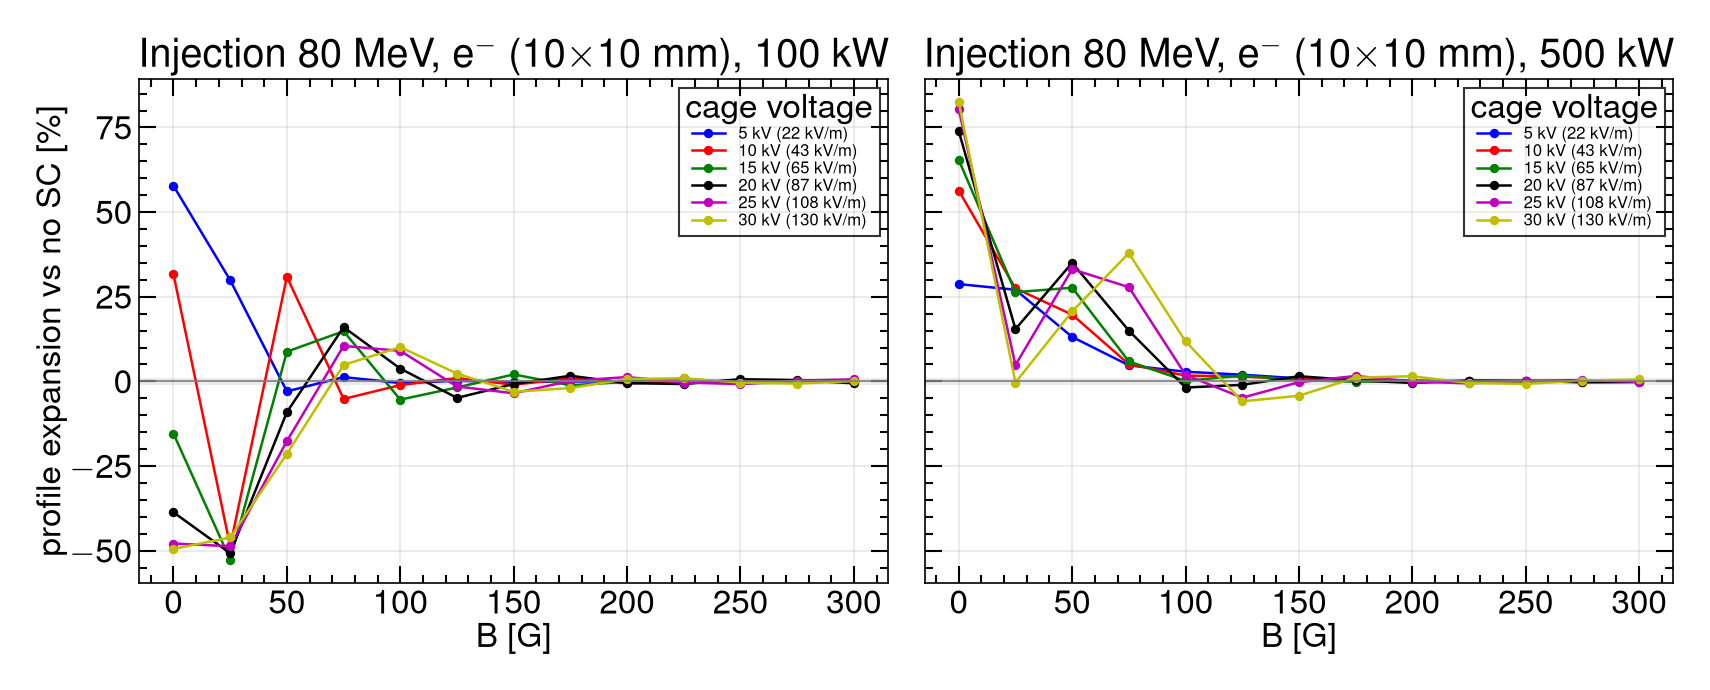
\includegraphics[width=0.98\textwidth]{csns_emode_voltage.png}
\caption{Relative expansion $\Delta$ of the electron profile as a
function of guiding field for cage voltages from $5$ to
$30\,\mathrm{kV}$, on the $10\,\mathrm{mm}$ injection beam.
At $B=0$ the $100\,\mathrm{kW}$ family crosses zero; the
$500\,\mathrm{kW}$ family does not.}
\label{fig:eV}
\end{figure}

The map $\sigma_m(\sigma_0)$ is not monotonic at $B=0$: a small beam
may appear larger or smaller than a large one, according to whether the
kick focuses or over-focuses. The Voitkiv $\mathrm{H}_2$ double
differential cross-section used by Virtual-IPM contributes a
$\sigma$-independent quadrature smear of $2.9$--$3.2\,\mathrm{mm}$
($\approx 2$--$2.5\,\mathrm{eV}$ per transverse axis), which is
$+40$--$48\%$ at $\sigma_0=3\,\mathrm{mm}$ and only $+1\%$ at
$20\,\mathrm{mm}$. One cyclotron period removes that smear
(Section~\ref{sec:Be}).

Along the energy ramp at $B=0$, a long bunch ($120\,\mathrm{ns}$) is
compressed and a short bunch ($20\,\mathrm{ns}$) is inflated. Both
errors become milder as $\beta$ rises, because the electrons spend less
time in the bunch: at $100\,\mathrm{kW}$ the $120\,\mathrm{ns}$ family
goes from $-46\%$ ($200\,\mathrm{MeV}$) to $-32\%$
($1.6\,\mathrm{GeV}$), and the $20\,\mathrm{ns}$ family from
$+77\%$ ($80\,\mathrm{MeV}$) to $+38\%$ ($1.2\,\mathrm{GeV}$). Energy
alone does not restore the profile.

\subsection{Ion collection}
\label{sec:ion}

Every ion case has $\Delta>0$. Figure~\ref{fig:isize} shows
$\sigma_m$ versus $\sigma_0$ at the design $0.1\,\mathrm{T}$ and
$100\,\mathrm{kW}$: every species and both rings lie above the
diagonal. Figure~\ref{fig:iexp} shows the growth with bunch charge and
the decrease with beam size required by Eq.~(\ref{eq:h}).

\begin{figure}[ht]
\centering
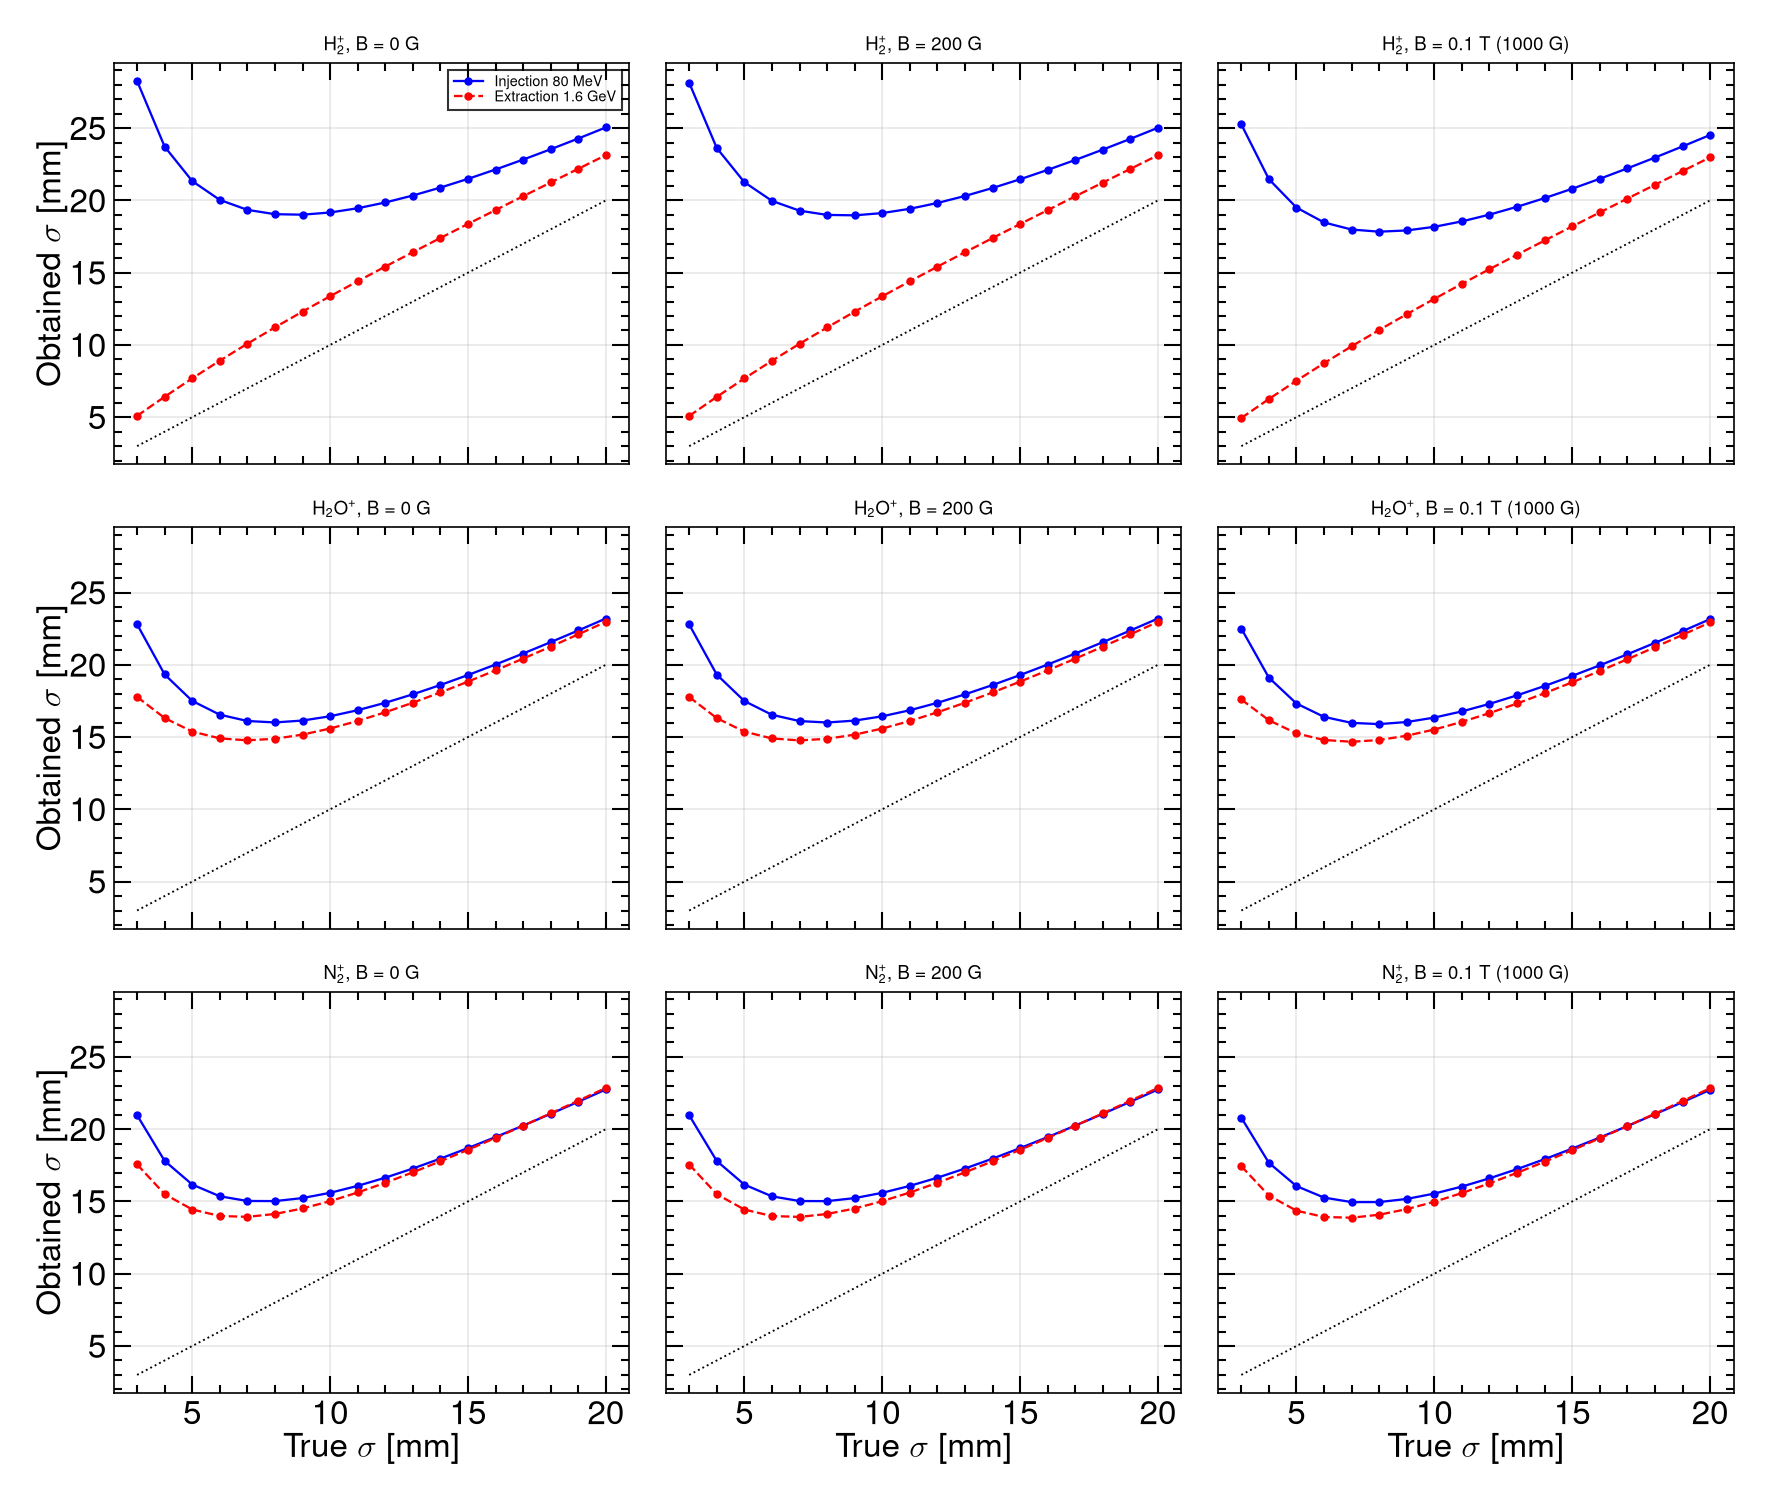
\includegraphics[width=0.98\textwidth]{csns_imode_size_obtained.png}
\caption{Ion-mode obtained width $\sigma_m$ versus true width
$\sigma_0$ at $0.1\,\mathrm{T}$ and $100\,\mathrm{kW}$. The dashed
line is $\sigma_m=\sigma_0$. Space charge inflates every point.}
\label{fig:isize}
\end{figure}

\begin{figure}[ht]
\centering
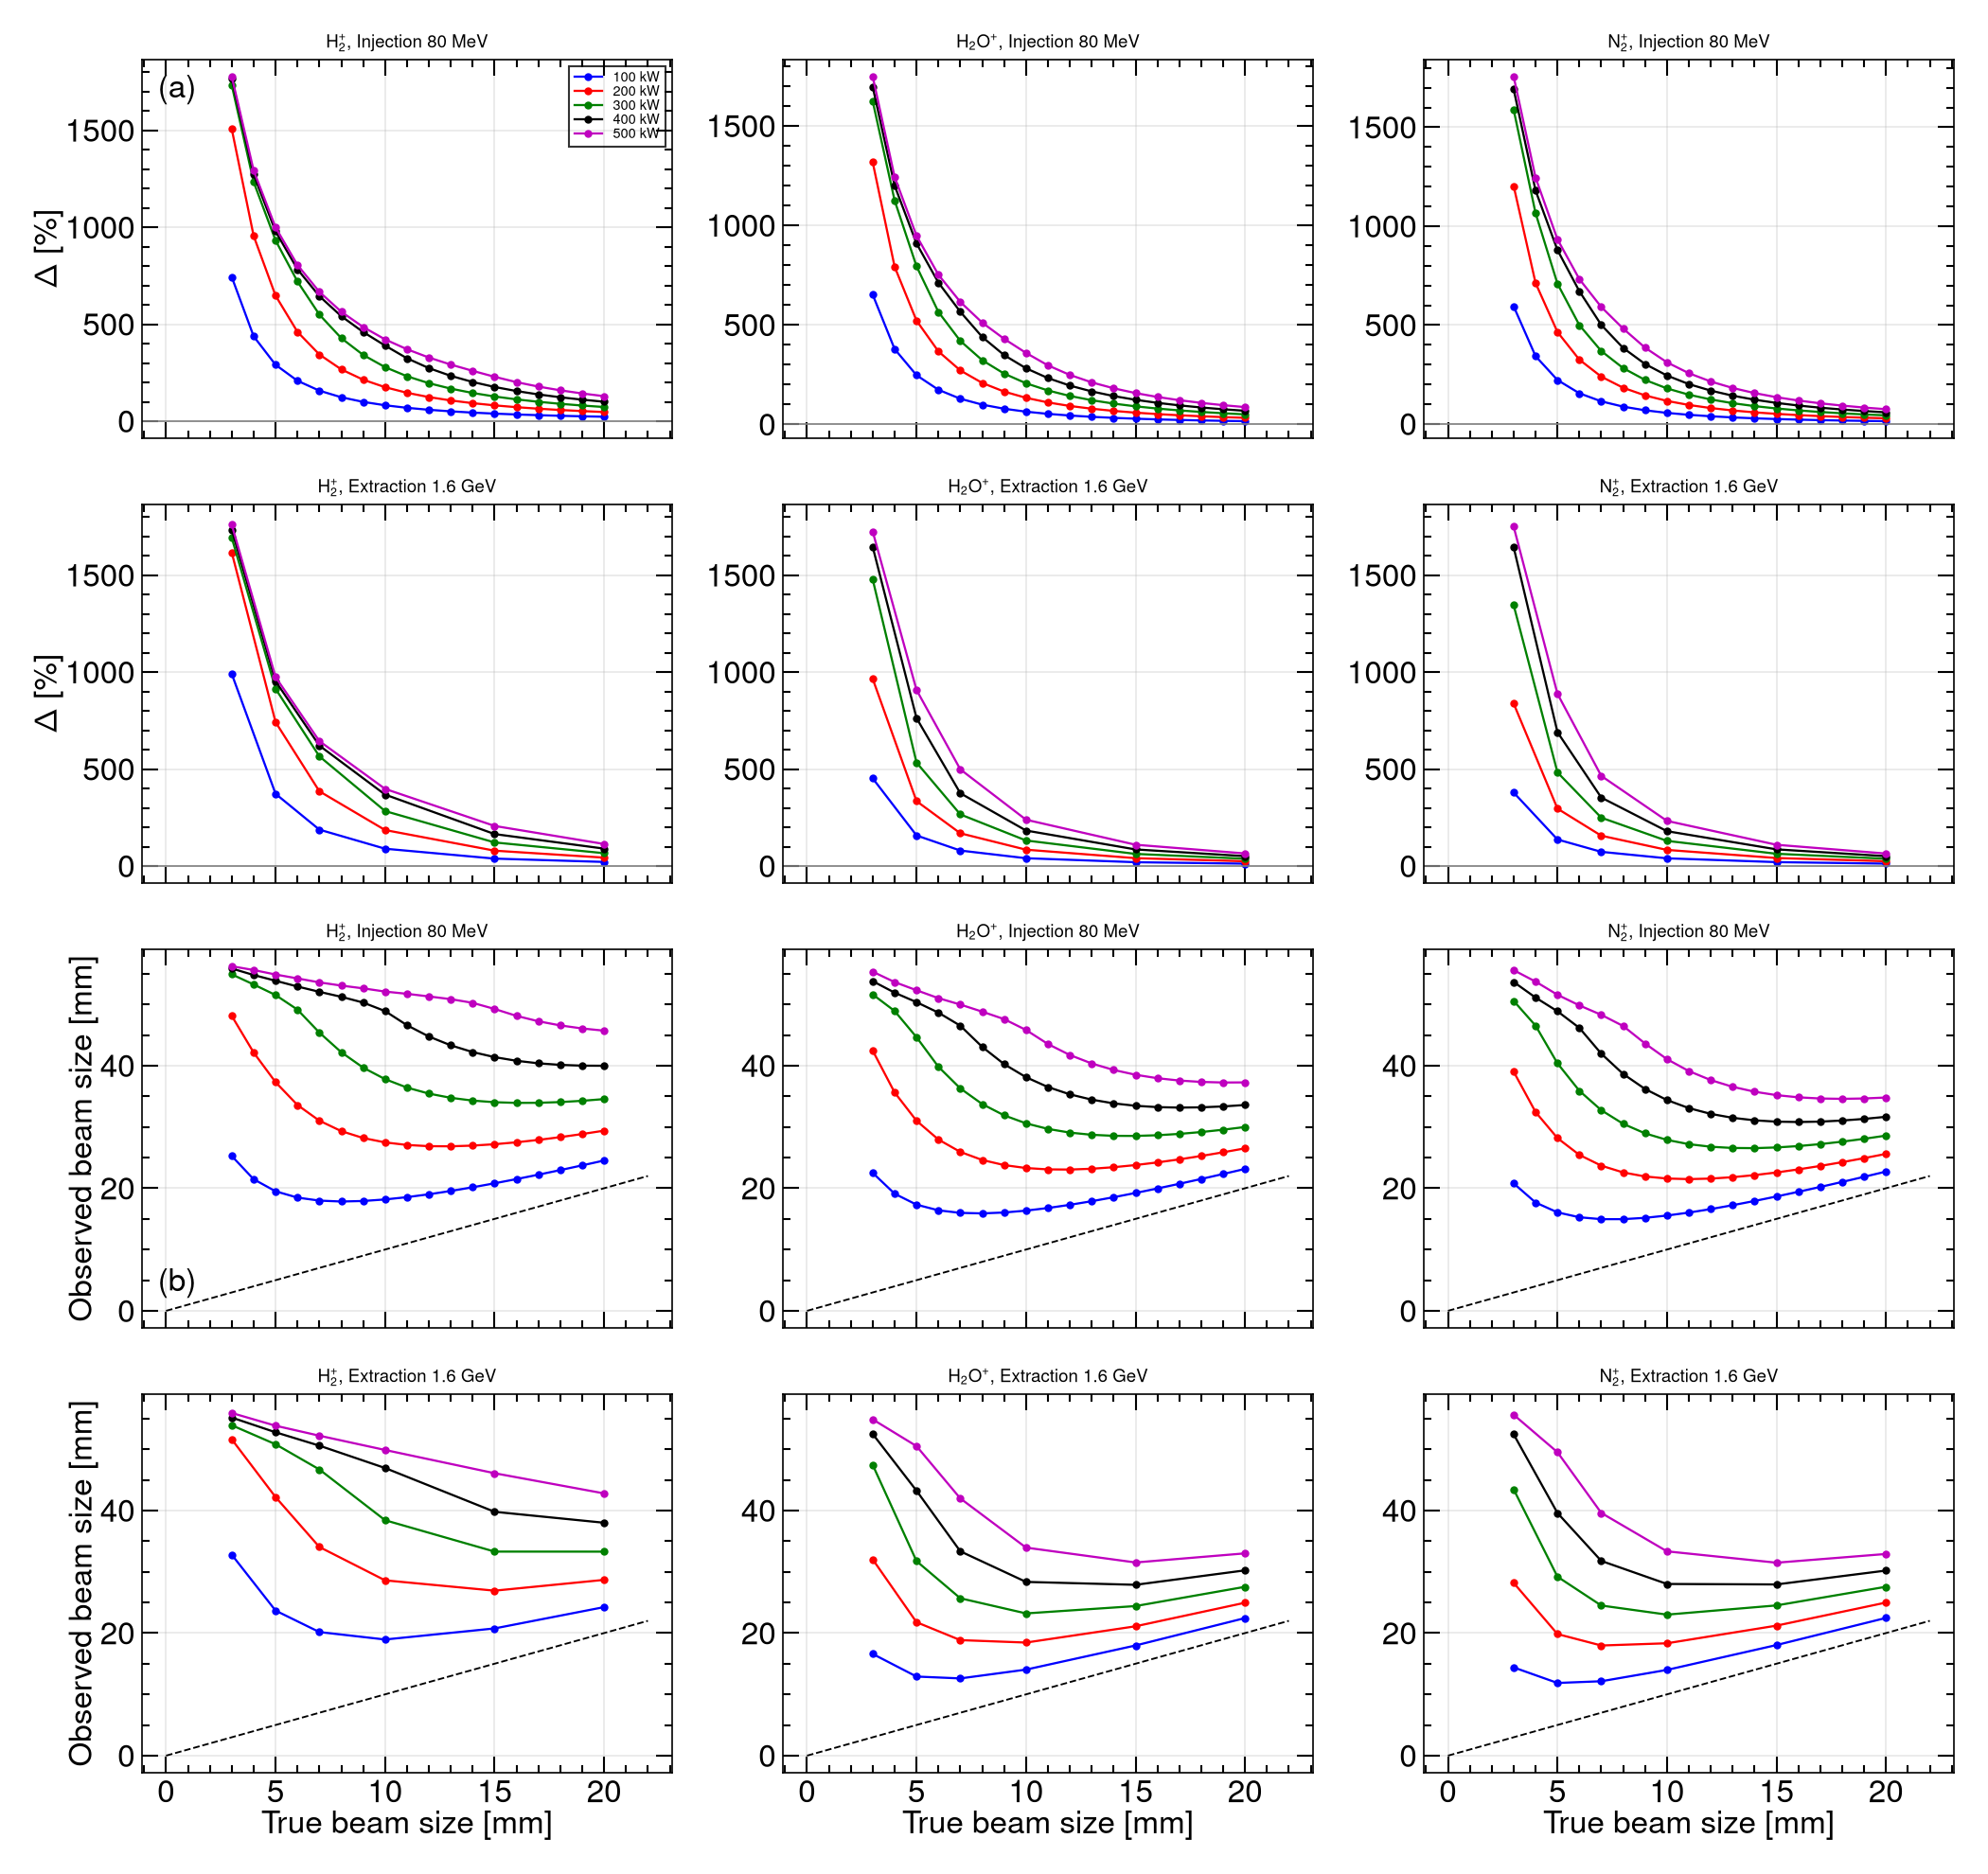
\includegraphics[width=0.98\textwidth]{csns_imode_size_expansion.png}
\caption{Ion-mode expansion versus true size at $0.1\,\mathrm{T}$ for
beam powers from $100$ to $500\,\mathrm{kW}$. The
$3\,\mathrm{mm}$/$500\,\mathrm{kW}$ family saturates on the cage wall
($\sigma_m\approx 56\,\mathrm{mm}$).}
\label{fig:iexp}
\end{figure}

For $\mathrm{H}_2^+$ at injection, $\sigma_0=10\,\mathrm{mm}$ and
$0.1\,\mathrm{T}$, the expansion grows from $+82\%$
($18.2\,\mathrm{mm}$) at $100\,\mathrm{kW}$ to $+175\%$, $+279\%$,
$+390\%$ and $+422\%$ ($52.1\,\mathrm{mm}$) at $200$, $300$, $400$ and
$500\,\mathrm{kW}$. Between $100$ and $400\,\mathrm{kW}$ the growth is
$\propto P^{1.12}$, consistent with the linear kick plus the
second-order term of
$\sigma_m^2=\sigma_0^2+\kappa N+\cdots$~\cite{Shiltsev2021}. At
$500\,\mathrm{kW}$ the profile reaches the $110\,\mathrm{mm}$
half-cage and the exponent saturates.

At extraction, with ions born in time with the bunch,
$10\,\mathrm{mm}$, $100\,\mathrm{kW}$ and $25\,\mathrm{kV}$, the
expansions are $+104\%$ ($\mathrm{H}_2^+$), $+41\%$
($\mathrm{H}_2\mathrm{O}^+$) and $+40\%$ ($\mathrm{N}_2^+$) at
$B=0$, in agreement with a reduced line-charge integration of the same
equations to $\pm 1\%$ absolute (Fig.~\ref{fig:kick}; model values
$+102\%$, $+40\%$ and $+39\%$). The $20\,\mathrm{ns}$ bunch is
impulsive, so $\mathrm{H}_2^+$ is the most distorted species. At
$500\,\mathrm{kW}$ the same family reaches $+408\%$, $+243\%$ and
$+235\%$. Between $\sigma_0=5$ and $20\,\mathrm{mm}$ at
$100\,\mathrm{kW}$, $\Delta\propto\sigma_0^{-1.84\ldots-2.01}$, the
impulsive $\sigma_0^{-2}$ of Eq.~(\ref{eq:h}) rather than the
continuous-beam $\sigma_0^{-1.5}$. Aligned extraction $\mathrm{H}_2^+$
widths at $0\,\mathrm{G}$ and $100\,\mathrm{kW}$ are listed in
Table~\ref{tab:esize}. A $3\,\mathrm{mm}$ extraction beam is already
unusable as a size measurement at $100\,\mathrm{kW}$. The most severe
case remains injection at $3\,\mathrm{mm}$ and $500\,\mathrm{kW}$,
where $\sigma_m\approx 56\,\mathrm{mm}$ ($+1700\%$) for all three
species.

\begin{table}[ht]
\centering
\caption{Aligned extraction, $\mathrm{H}_2^+$, $0\,\mathrm{G}$,
$100\,\mathrm{kW}$, $25\,\mathrm{kV}$: obtained width and expansion
versus true size.}
\label{tab:esize}
\begin{tabular}{lcccccc}
\hline\hline
$\sigma_0$\,(mm) & 3 & 5 & 7 & 10 & 15 & 20 \\
\hline
$\sigma_m$\,(mm) & 38.2 & 26.8 & 22.4 & 20.4 & 21.7 & 24.9 \\
$\Delta$\,(\%)   & $+1172$ & $+435$ & $+219$ & $+104$ & $+44$ & $+24$ \\
\hline\hline
\end{tabular}
\end{table}

\begin{figure}[ht]
\centering
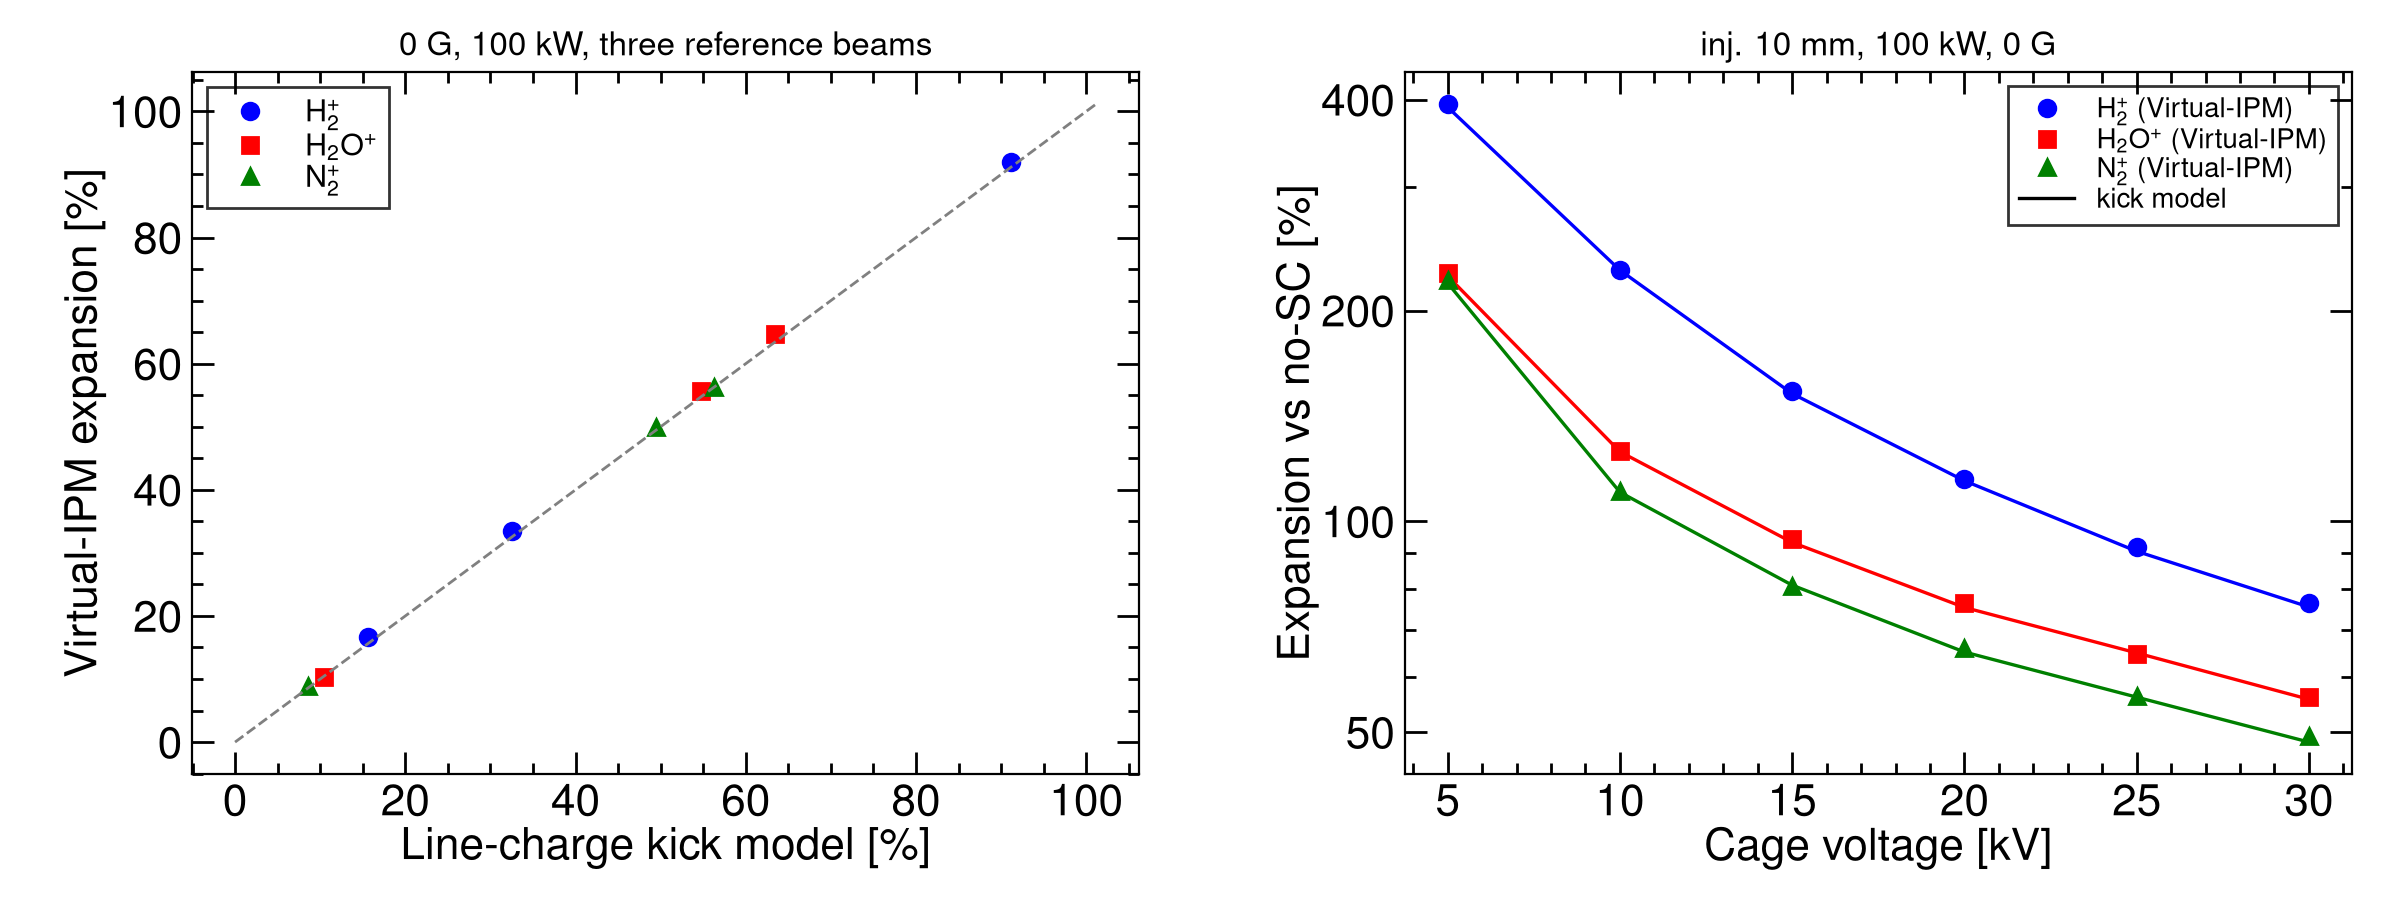
\includegraphics[width=0.98\textwidth]{csns_review_imode_model.png}
\caption{Left: ion-mode expansion at $0\,\mathrm{G}$ and
$100\,\mathrm{kW}$, reduced kick model versus Virtual-IPM. Right:
cage-voltage scan at $0\,\mathrm{G}$. Agreement is
$\pm 1\%$ absolute.}
\label{fig:kick}
\end{figure}

Species ordering follows the mixed regime. At injection,
$10\,\mathrm{mm}$, $0\,\mathrm{G}$ and $100\,\mathrm{kW}$ the
expansions are $+92\%$ ($\mathrm{H}_2^+$), $+65\%$
($\mathrm{H}_2\mathrm{O}^+$) and $+56\%$ ($\mathrm{N}_2^+$): lighter
ions expand more, but less than a pure $M^{-1/2}$ law because
$\mathrm{H}_2^+$ leaves during the $120\,\mathrm{ns}$ bunch. Painted
injection ($25\,\mathrm{mm}$) is milder ($+17\%$, $+10\%$, $+9\%$). A
second extraction bunch, still in the cage when the heavy ions arrive,
adds a few points of extra width (single-bunch $+36\%$ and $+29\%$
versus three-bunch $+41\%$ and $+40\%$ for $\mathrm{H}_2\mathrm{O}^+$
and $\mathrm{N}_2^+$); $\mathrm{H}_2^+$ does not see that bunch
($+104\%$ either way). At commissioning power, aligned extraction
$\mathrm{H}_2^+$ ($10\,\mathrm{mm}$, $0\,\mathrm{G}$) is already
$+19\%$ at $20\,\mathrm{kW}$ and $+82\%$ at $80\,\mathrm{kW}$. These
magnitudes are of the same order as the operational ion-mode biases
reported at J-PARC RCS ($20$--$30\%$ wider than the
MWPM)~\cite{Satou2010} and at the Fermilab
Booster~\cite{Shiltsev2021}.

\section{Mitigation}
\label{sec:mit}

\subsection{Magnetic confinement of electrons}
\label{sec:Be}

Figure~\ref{fig:eB} shows the electron expansion versus $B$ for the
three reference beams and $100$--$500\,\mathrm{kW}$. The curves
oscillate through focusing and over-kick. Painted injection recovers
first; extraction and the $10\,\mathrm{mm}$ injection core still
oscillate through $150$--$250\,\mathrm{G}$. At $300\,\mathrm{G}$ every
family has settled inside $\pm 1\%$ (Fig.~\ref{fig:eBtail}).

\begin{figure}[ht]
\centering
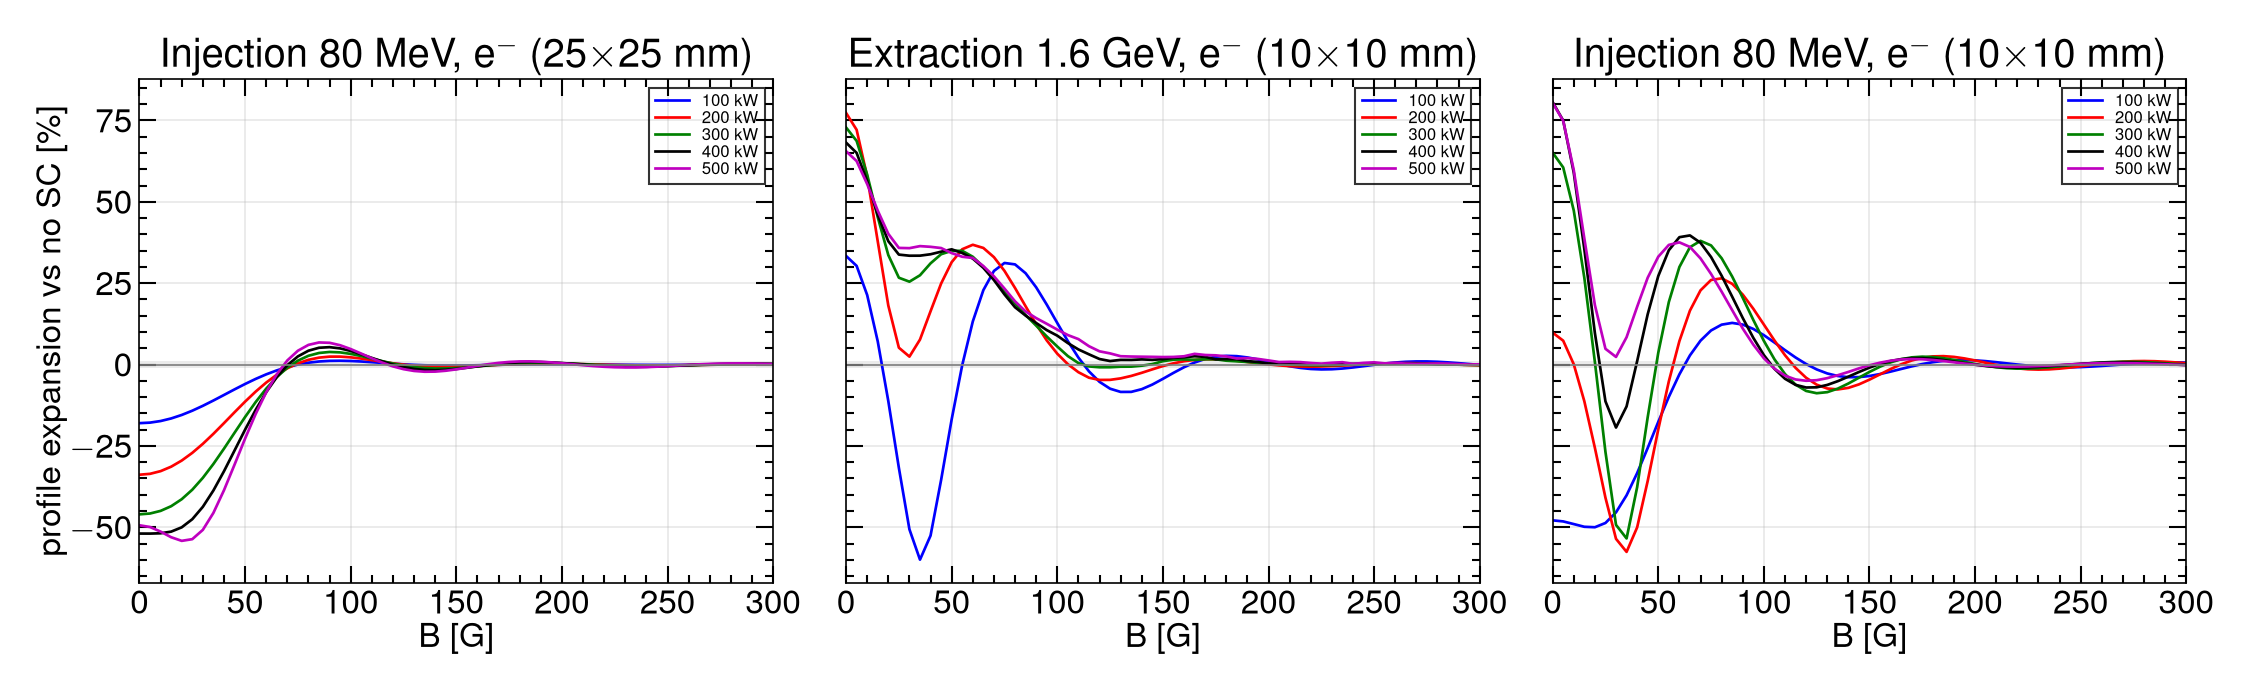
\includegraphics[width=0.98\textwidth]{csns_emode_bscan300.png}
\caption{Electron-mode expansion versus guiding field, $0$--$300\,\mathrm{G}$,
for painted injection ($25\,\mathrm{mm}$), extraction
($10\,\mathrm{mm}$) and the $10\,\mathrm{mm}$ injection core, at
$100$--$500\,\mathrm{kW}$. The grey band is $\pm 1\%$.}
\label{fig:eB}
\end{figure}

\begin{figure}[ht]
\centering
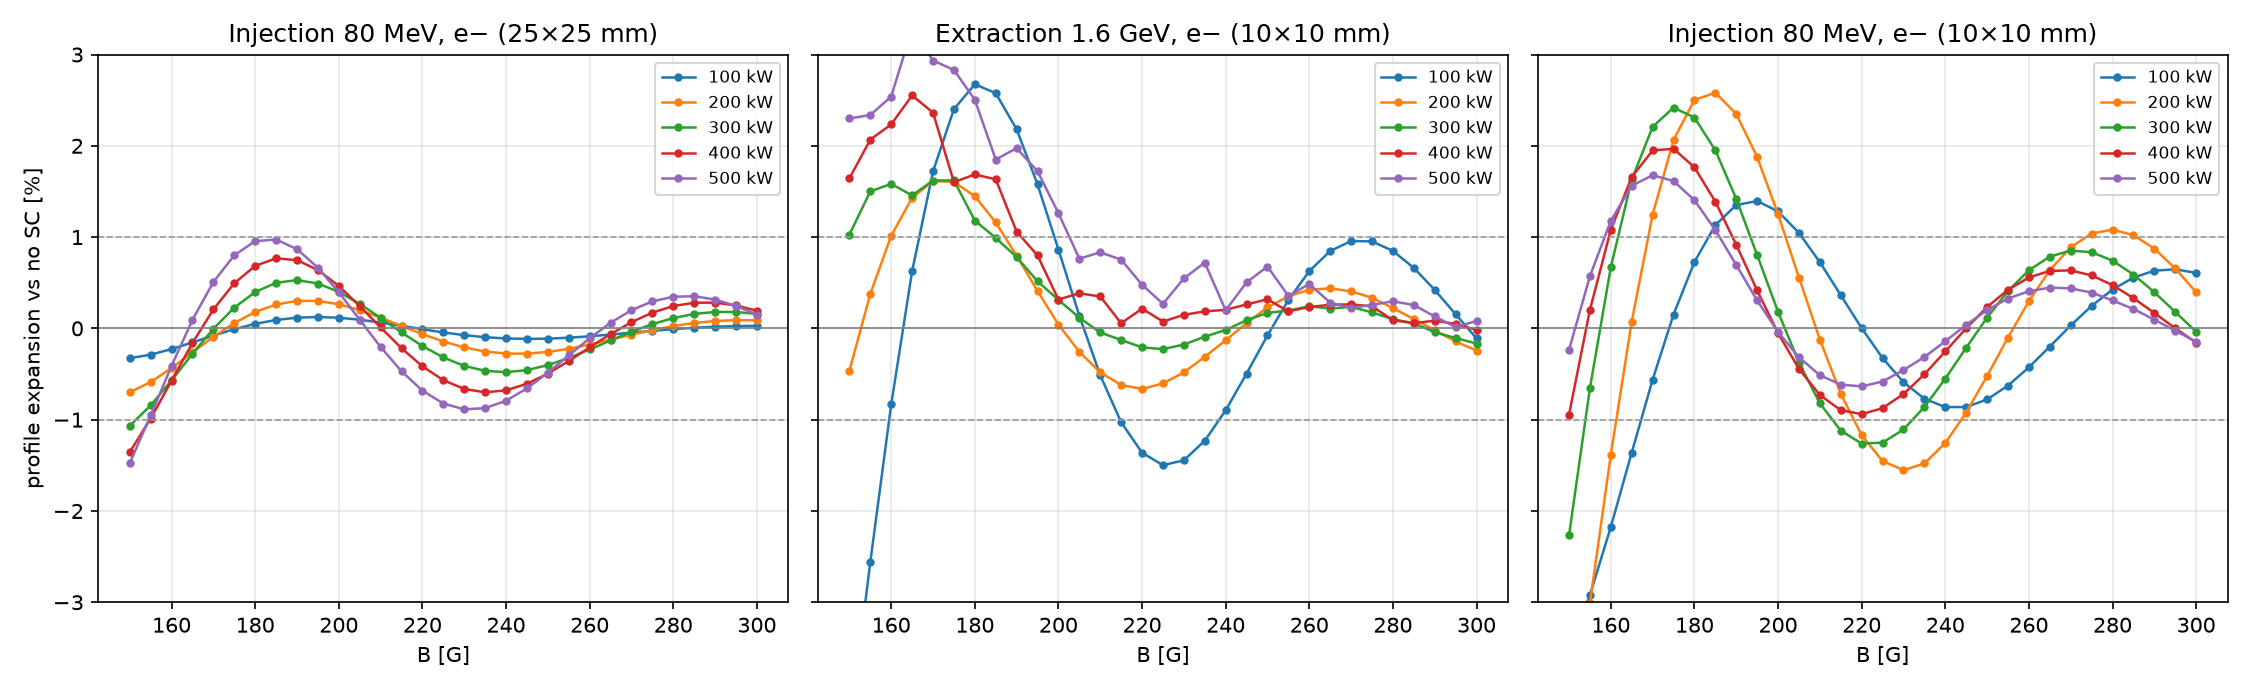
\includegraphics[width=0.98\textwidth]{csns_emode_bscan300_tail.png}
\caption{As Fig.~\ref{fig:eB}, $150$--$300\,\mathrm{G}$,
$\pm 3\%$ vertical scale. At $300\,\mathrm{G}$ every family lies
inside $\pm 1\%$.}
\label{fig:eBtail}
\end{figure}

\clearpage
Figures~\ref{fig:eB} and~\ref{fig:eBtail} do not fall monotonically:
$\Delta(B)$ oscillates through focusing ($\Delta<0$) and over-kick
($\Delta>0$). Figure~\ref{fig:cyc} identifies that oscillation as the
cyclotron phase of a nearly impulsive space-charge kick.

\begin{figure}[!t]
\centering
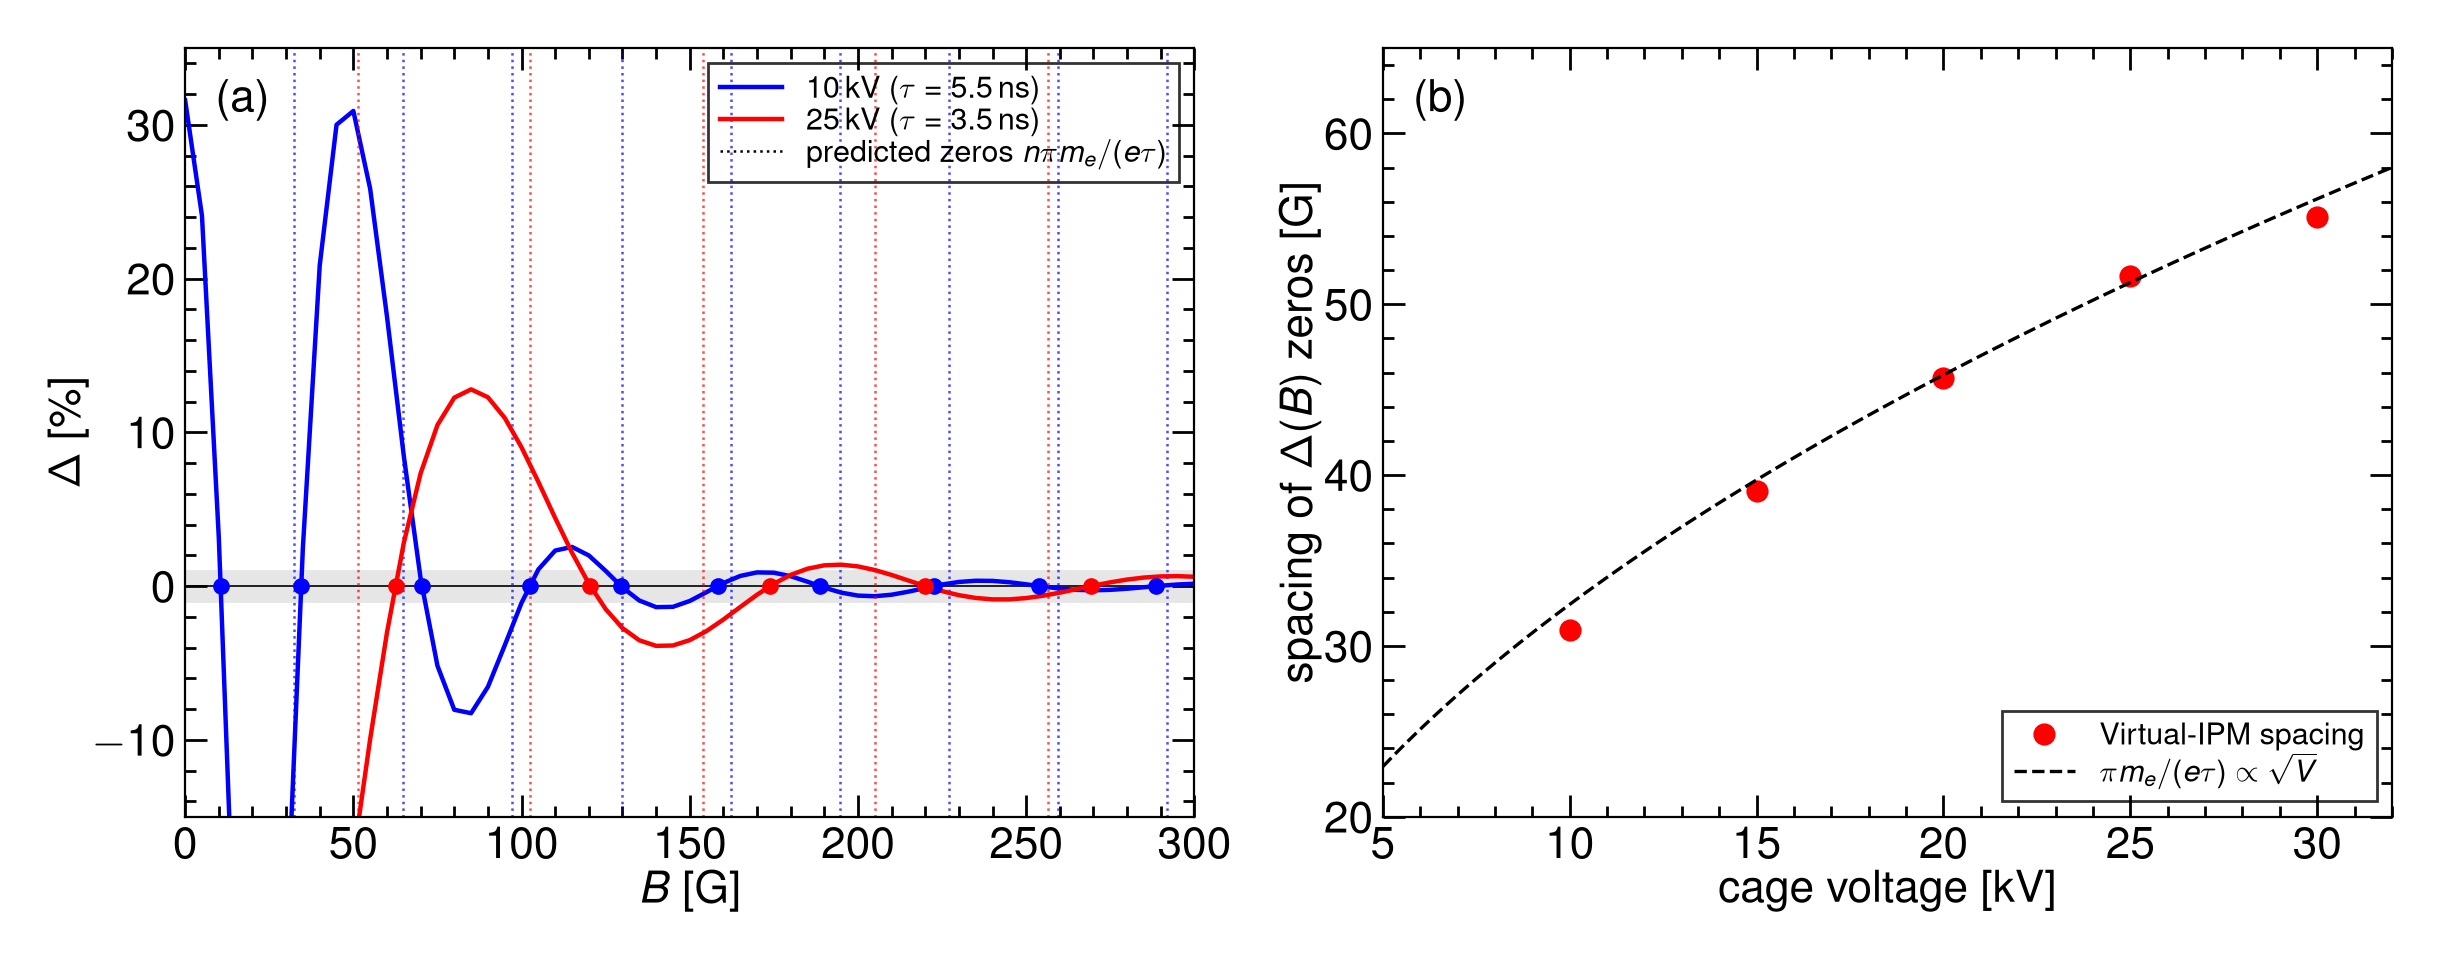
\includegraphics[width=0.98\textwidth]{csns_review_emode_cyclotron.png}
\caption{(a)~Relative expansion $\Delta$ versus guiding field at two
cage voltages ($100\,\mathrm{kW}$, $10\,\mathrm{mm}$ injection).
Dotted vertical lines (colour-matched to the curves) are the predicted
zeros $B_n=n\pi m_e/(e\tau)$; circles are the simulated crossings. The
grey band is $\pm 1\%$. The $25\,\mathrm{kV}$ point at $B=0$
($\Delta=-48\%$) is off-scale. (b)~Mean spacing of those zeros versus
cage voltage, compared with $\pi m_e/(e\tau)\propto\sqrt{V}$ (no free
parameter).}
\label{fig:cyc}
\end{figure}

An electron born on a $10\,\mathrm{mm}$ beam leaves the bunch in
$\lesssim 1\,\mathrm{ns}$ and then drifts the remaining
$\tau\simeq 3.5\,\mathrm{ns}$ ($25\,\mathrm{kV}$) in the uniform cage
field. The transverse impulse $\Delta v$ acquired inside the bunch is
converted into cyclotron motion at $\omega_c=eB/m_e$. The displacement
at the collector is $(\Delta v/\omega_c)\sin(\omega_c\tau)$ and
therefore vanishes whenever the electron completes an integer number of
half-turns, $\omega_c\tau=n\pi$ ($n=1,2,\ldots$). Those fields are
exactly the equally spaced zeros $B_n=n\,\pi m_e/(e\tau)$ of
Eq.~(\ref{eq:dB}). Because $\tau\propto V^{-1/2}$ in a uniform field,
the spacing itself scales as $\sqrt{V}$. The amplitude of each
successive lobe falls as $1/B$ (the $1/\omega_c$ prefactor). Magnetic
mitigation is the decay of that envelope, not the choice of a particular
zero: a zero can be moved by a few kilovolts or a change of orbit,
whereas the envelope is a property of $B$.

Panel~(a) is a $5\,\mathrm{G}$-step scan at $100\,\mathrm{kW}$ and
$10\,\mathrm{mm}$ injection, drawn at $10$ and $25\,\mathrm{kV}$.
Vertical dotted lines are the predicted zeros
$B_n=n\pi m_e/(e\tau)$ for each voltage; filled circles mark the
Virtual-IPM crossings. The $10\,\mathrm{kV}$ curve oscillates faster
because the flight is longer ($\tau=5.51\,\mathrm{ns}$ versus
$3.48\,\mathrm{ns}$), so a given phase $n\pi$ is reached at a weaker
$B$. The first $25\,\mathrm{kV}$ point, $\Delta=-48\%$ at $B=0$, lies
below the frame. At $25\,\mathrm{kV}$ the remaining lobes sit near
$85$, $140$, $195$, $240$ and $295\,\mathrm{G}$ with amplitudes $13$,
$4$, $1.4$, $0.9$ and $0.6\%$.

Panel~(b) extracts the mean spacing between successive zeros at five
cage voltages and compares it with $\pi m_e/(e\tau)$
(Table~\ref{tab:cyc}). The points follow the $\sqrt{V}$ curve to
$\le 5\%$ from $10$ to $30\,\mathrm{kV}$ with no free parameter. That
is the evidence that the oscillation in Figs.~\ref{fig:eB}
and~\ref{fig:eBtail} is the cyclotron phase, and it is why
$300\,\mathrm{G}$---the first field at which the envelope itself lies
inside $\pm 1\%$ at every power---is the operating point rather than
any particular zero.

\begin{table}[!ht]
\centering
\caption{Electron time of flight from the cage mid-plane and the
spacing of $\Delta(B)$ zeros ($5\,\mathrm{G}$ voltage scan, injection
$10\,\mathrm{mm}$, $100\,\mathrm{kW}$). The prediction is
Eq.~(\ref{eq:dB}) with $\tau=\sqrt{2 d m_e/(eE)}$ and
$d=115.5\,\mathrm{mm}$.}
\label{tab:cyc}
{\small
\begin{tabular}{cccc}
\hline\hline
Cage voltage & ToF $\tau$ & $\Delta B$ predicted & $\Delta B$ simulated \\
\hline
$10\,\mathrm{kV}$ & $5.51\,\mathrm{ns}$ & $32.4\,\mathrm{G}$ & $30.9\,\mathrm{G}$ \\
$15\,\mathrm{kV}$ & $4.50\,\mathrm{ns}$ & $39.7\,\mathrm{G}$ & $39.1\,\mathrm{G}$ \\
$20\,\mathrm{kV}$ & $3.89\,\mathrm{ns}$ & $45.9\,\mathrm{G}$ & $45.7\,\mathrm{G}$ \\
$25\,\mathrm{kV}$ & $3.48\,\mathrm{ns}$ & $51.3\,\mathrm{G}$ & $51.7\,\mathrm{G}$ \\
$30\,\mathrm{kV}$ & $3.18\,\mathrm{ns}$ & $56.2\,\mathrm{G}$ & $55.1\,\mathrm{G}$ \\
\hline\hline
\end{tabular}
}
\end{table}

Table~\ref{tab:Bth} lists the smallest field after which
$\lvert\Delta\rvert$ remains below $1\%$, together with the residual at
$300\,\mathrm{G}$. Painted injection is restored first. The last curve
to settle is the $10\,\mathrm{mm}$ injection core at $200\,\mathrm{kW}$
($290\,\mathrm{G}$). A field of $300\,\mathrm{G}$ keeps every power at
$\lvert\Delta\rvert\lesssim 1\%$.

\begin{table}[ht]
\centering
\caption{Smallest guiding field after which $\lvert\Delta\rvert\le 1\%$
for the remainder of the $0$--$300\,\mathrm{G}$ grid. The residual at
$300\,\mathrm{G}$ is given in parentheses.}
\label{tab:Bth}
{\small
\begin{tabular}{lccccc}
\hline\hline
Beam & 100\,kW & 200\,kW & 300\,kW & 400\,kW & 500\,kW \\
\hline
Inj.\ $25\,\mathrm{mm}$
  & $105\,\mathrm{G}$ ($+0.03\%$)
  & $115\,\mathrm{G}$ ($+0.09\%$)
  & $155\,\mathrm{G}$ ($+0.16\%$)
  & $155\,\mathrm{G}$ ($+0.19\%$)
  & $155\,\mathrm{G}$ ($+0.15\%$) \\
Ext.\ $10\,\mathrm{mm}$
  & $240\,\mathrm{G}$ ($-0.11\%$)
  & $190\,\mathrm{G}$ ($-0.24\%$)
  & $185\,\mathrm{G}$ ($-0.17\%$)
  & $195\,\mathrm{G}$ ($-0.02\%$)
  & $205\,\mathrm{G}$ ($+0.08\%$) \\
Inj.\ $10\,\mathrm{mm}$
  & $210\,\mathrm{G}$ ($+0.61\%$)
  & $290\,\mathrm{G}$ ($+0.40\%$)
  & $235\,\mathrm{G}$ ($-0.04\%$)
  & $190\,\mathrm{G}$ ($-0.16\%$)
  & $190\,\mathrm{G}$ ($-0.15\%$) \\
\hline\hline
\end{tabular}
}
\end{table}

The same $300\,\mathrm{G}$ point holds when the remaining axes are
varied. From $200\,\mathrm{G}$ the obtained-versus-true plot lies on
the diagonal except at $3\,\mathrm{mm}$ (Fig.~\ref{fig:esize}). At
$300\,\mathrm{G}$, injection at $3\,\mathrm{mm}$ is still $+1\%$
($100\,\mathrm{kW}$) to $+4\%$ ($500\,\mathrm{kW}$); $0.1\,\mathrm{T}$
places $3$, $10$ and $20\,\mathrm{mm}$ on the diagonal at every power
($\lvert\Delta\rvert\le 0.05\%$). At $300\,\mathrm{G}$ and
$10$--$25\,\mathrm{kV}$, both $100$ and $500\,\mathrm{kW}$ remain
$\lesssim 1\%$. Higher $V$ requires slightly more $B$ at
$100\,\mathrm{kW}$ ($150\,\mathrm{G}$ at $10\,\mathrm{kV}$ to
$210\,\mathrm{G}$ at $25\,\mathrm{kV}$) because $\tau$ is shorter and
the first lobes move out; $500\,\mathrm{kW}$ recovers earlier at every
voltage. Along the energy ramp, $300\,\mathrm{G}$ and
$100\,\mathrm{kW}$ give $\lvert\Delta\rvert\le 0.5\%$ from
$80\,\mathrm{MeV}$ to $1.6\,\mathrm{GeV}$ for both $120\,\mathrm{ns}$
and $20\,\mathrm{ns}$ bunches. At commissioning powers
($20$/$50$/$80\,\mathrm{kW}$) and $300\,\mathrm{G}$ the residuals are
$+0.00$/$+0.01$/$+0.02\%$ (painted injection),
$+0.28$/$+0.56$/$+0.18\%$ (extraction $10\,\mathrm{mm}$) and
$+0.11$/$+0.29$/$+0.49\%$ (injection $10\,\mathrm{mm}$).

A few millimetres of vertical orbit offset change $\Delta$ by a few
percent at $B=0$ and by $\lesssim 1\%$ at $300\,\mathrm{G}$; the
$1\%$ threshold moves by at most $\sim 10\,\mathrm{G}$. A horizontal
offset is a translation of a uniform cage and does not change the
width. The space-charge-induced centroid shift falls as $1/B$
(the $\mathbf{E}\times\mathbf{B}$ / polarisation drift of
Ref.~\cite{Vilsmeier2019}): $0.9\,\mathrm{mm}$ at $100\,\mathrm{G}$ to
$0.2\,\mathrm{mm}$ at $300\,\mathrm{G}$ on the extraction beam.

\begin{figure}[ht]
\centering
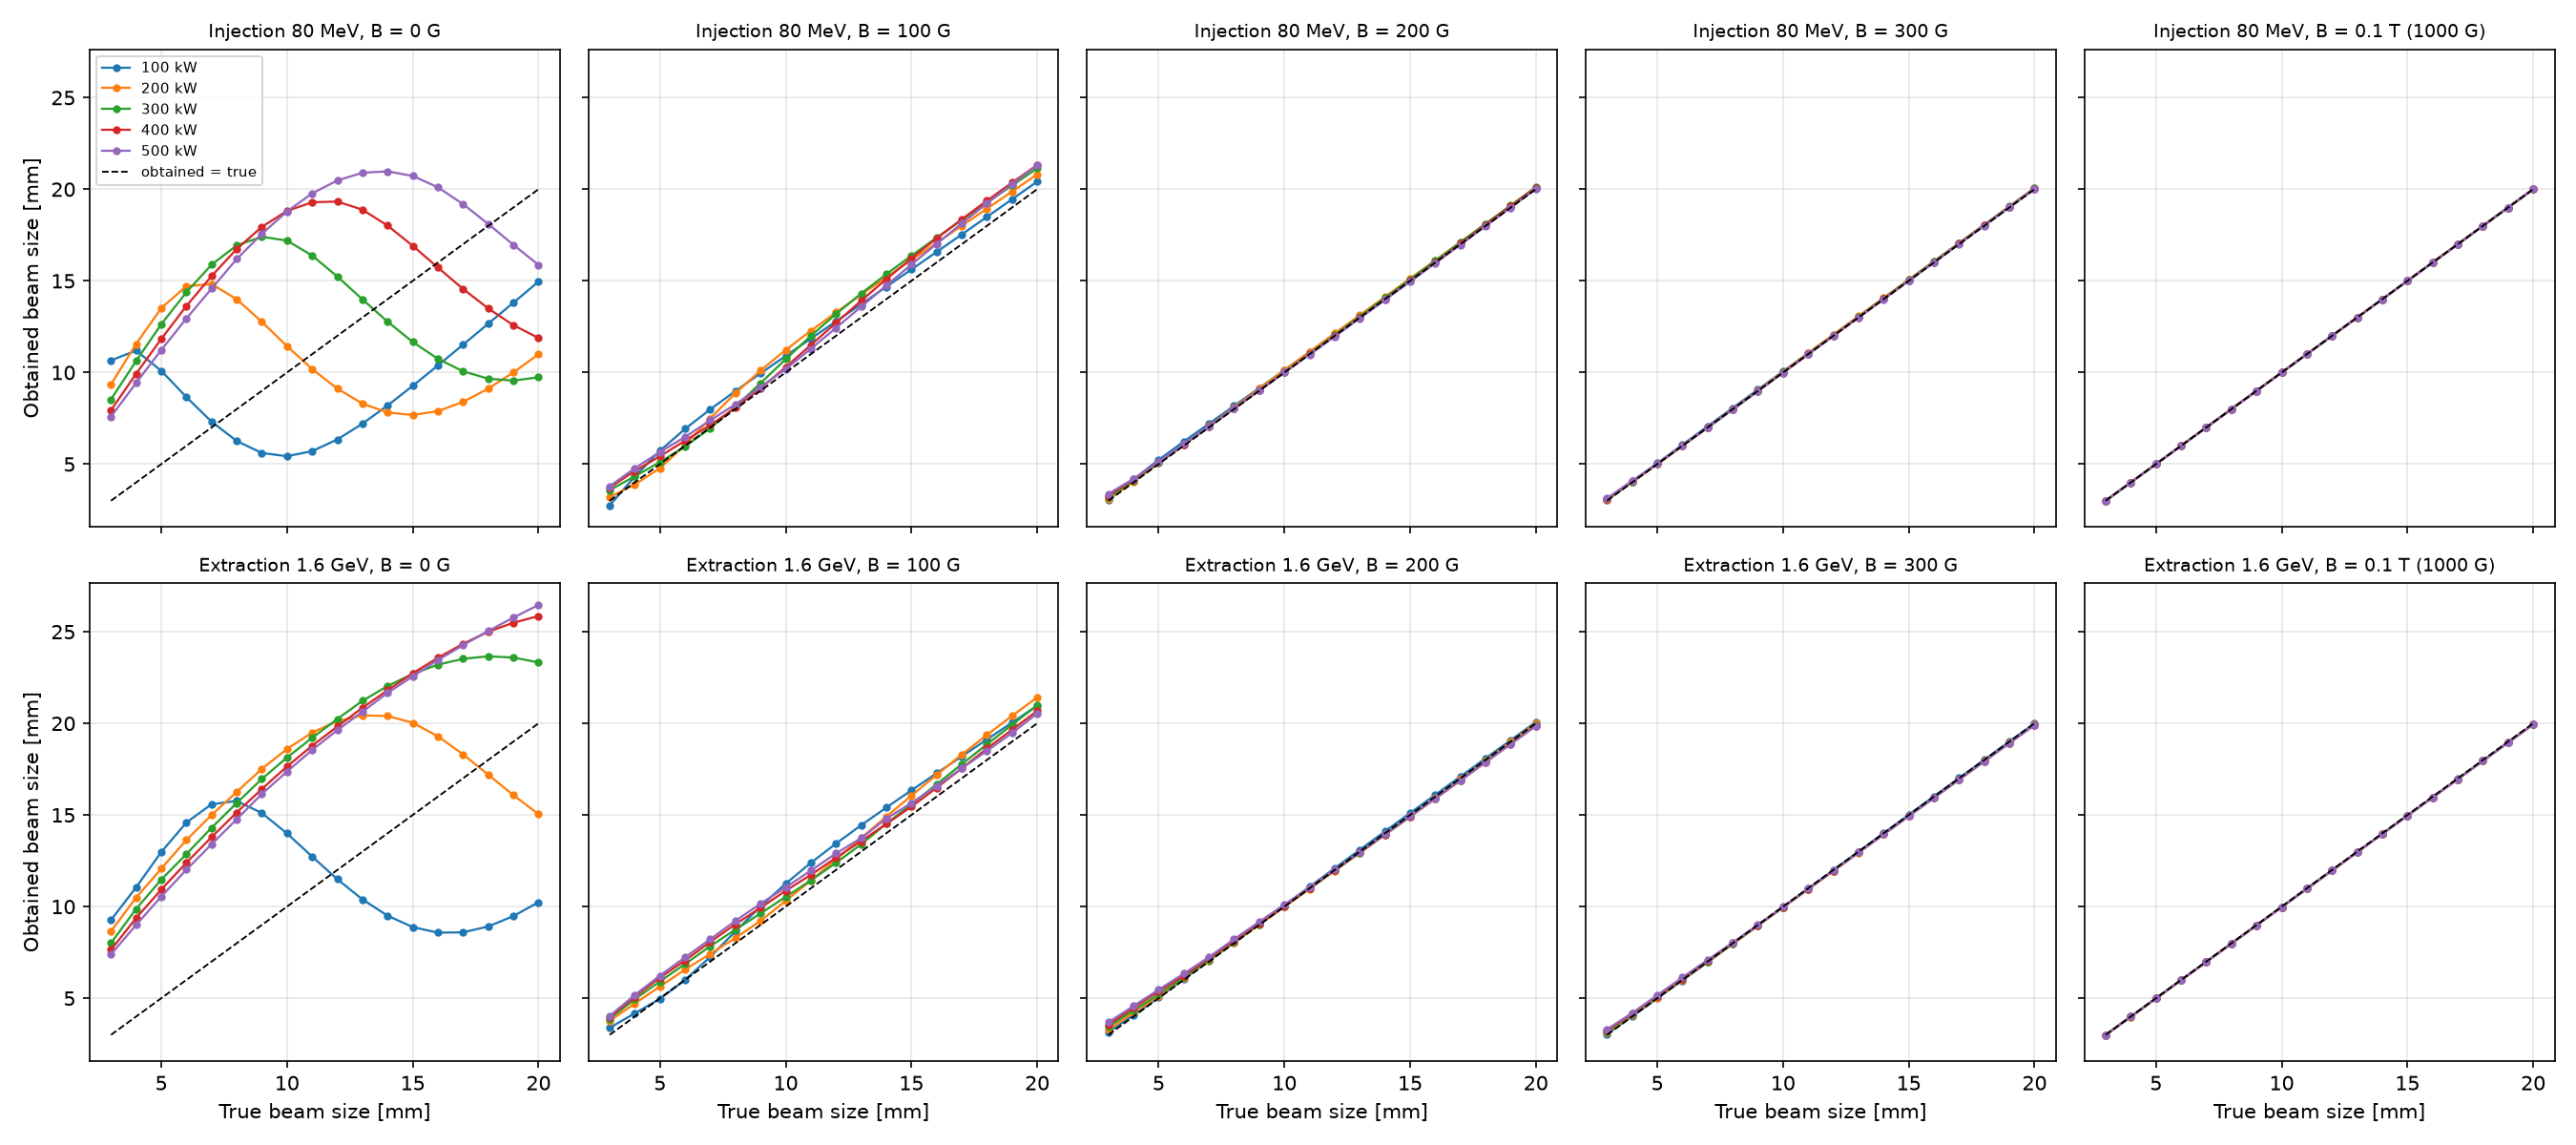
\includegraphics[width=0.98\textwidth]{csns_emode_size_obtained.png}
\caption{Electron-mode obtained width versus true width. From
$200\,\mathrm{G}$ the points lie on the diagonal; $0.1\,\mathrm{T}$
includes the $3\,\mathrm{mm}$ beams.}
\label{fig:esize}
\end{figure}

Thus $B=300\,\mathrm{G}$ reduces an electron-mode error of tens of
percent (and the wrong sign at $100\,\mathrm{kW}$ and high $V$) to
$\lesssim 1\%$. The design $0.1\,\mathrm{T}$ provides a factor-of-three
margin and is the appropriate field for a $3\,\mathrm{mm}$ beam. The
CSNS magnet ($0.2\,\mathrm{T}$) is not the limiting device. The SNS
ring IPM was designed for $300\,\mathrm{G}$ at twenty-five times this
bunch charge, with an estimated residual of about
$7\%$~\cite{Bartkoski2014}; a residual $\lesssim 1\%$ at CSNS is the
expected scaling. The CERN PS beam-gas ionization monitor operates at
$200\,\mathrm{mT}$ for LHC-type bunches~\cite{Levasseur2026}, at the
high-field end of the same scaling.

\subsection{Cage voltage}
\label{sec:V}

For electrons at $B=0$, voltage is not a size correction: it can reverse
the sign of $\Delta$ at $100\,\mathrm{kW}$ and cannot reverse it at
$500\,\mathrm{kW}$ (Section~\ref{sec:e0}). Once
$B\ge 300\,\mathrm{G}$ the design $25\,\mathrm{kV}$ already lies inside
$1\%$, so the voltage may be chosen for collection efficiency and
detector operation.

For ions, a higher $V$ shortens $\tau_2$ and reduces the integrated
kick, as at ISIS (broadening $\propto 1/E$)~\cite{Pine2006}.
Table~\ref{tab:iV} gives $\mathrm{H}_2^+$ at injection,
$10\,\mathrm{mm}$, $100\,\mathrm{kW}$ and $0.1\,\mathrm{T}$. Aligned
extraction $\mathrm{H}_2^+$ ($10\,\mathrm{mm}$, $100\,\mathrm{kW}$,
$0\,\mathrm{G}$) falls from $+280\%$ at $5\,\mathrm{kV}$ to
$+104\%$ at $25\,\mathrm{kV}$ and $+93\%$ at $30\,\mathrm{kV}$. The
$0\,\mathrm{G}$ scan scales as $V^{-0.92}$ ($\mathrm{H}_2^+$) and
$V^{-0.77}$ ($\mathrm{H}_2\mathrm{O}^+$). Extrapolating
$V^{-0.9}$, a $10\%$ bias on the $10\,\mathrm{mm}$ injection beam at
$100\,\mathrm{kW}$ would require approximately $380\,\mathrm{kV}$
across the cage, which is not a practical path. ESS can operate an ion
IPM at $300\,\mathrm{kV\,m^{-1}}$ because its bunches are weaker by
about $5000$~\cite{Marroncle2023}; that choice does not transfer to
CSNS. Figure~\ref{fig:iV} shows that the ion expansion remains positive
at every scanned voltage.

\begin{table}[ht]
\centering
\caption{$\mathrm{H}_2^+$ injection, $10\,\mathrm{mm}$,
$100\,\mathrm{kW}$, $0.1\,\mathrm{T}$: expansion versus cage voltage.}
\label{tab:iV}
\begin{tabular}{lcccccc}
\hline\hline
$V$\,(kV) & 5 & 10 & 15 & 20 & 25 & 30 \\
\hline
$\Delta$\,(\%) & $+198$ & $+168$ & $+126$ & $+100$ & $+82$ & $+70$ \\
\hline\hline
\end{tabular}
\end{table}

\begin{figure}[ht]
\centering
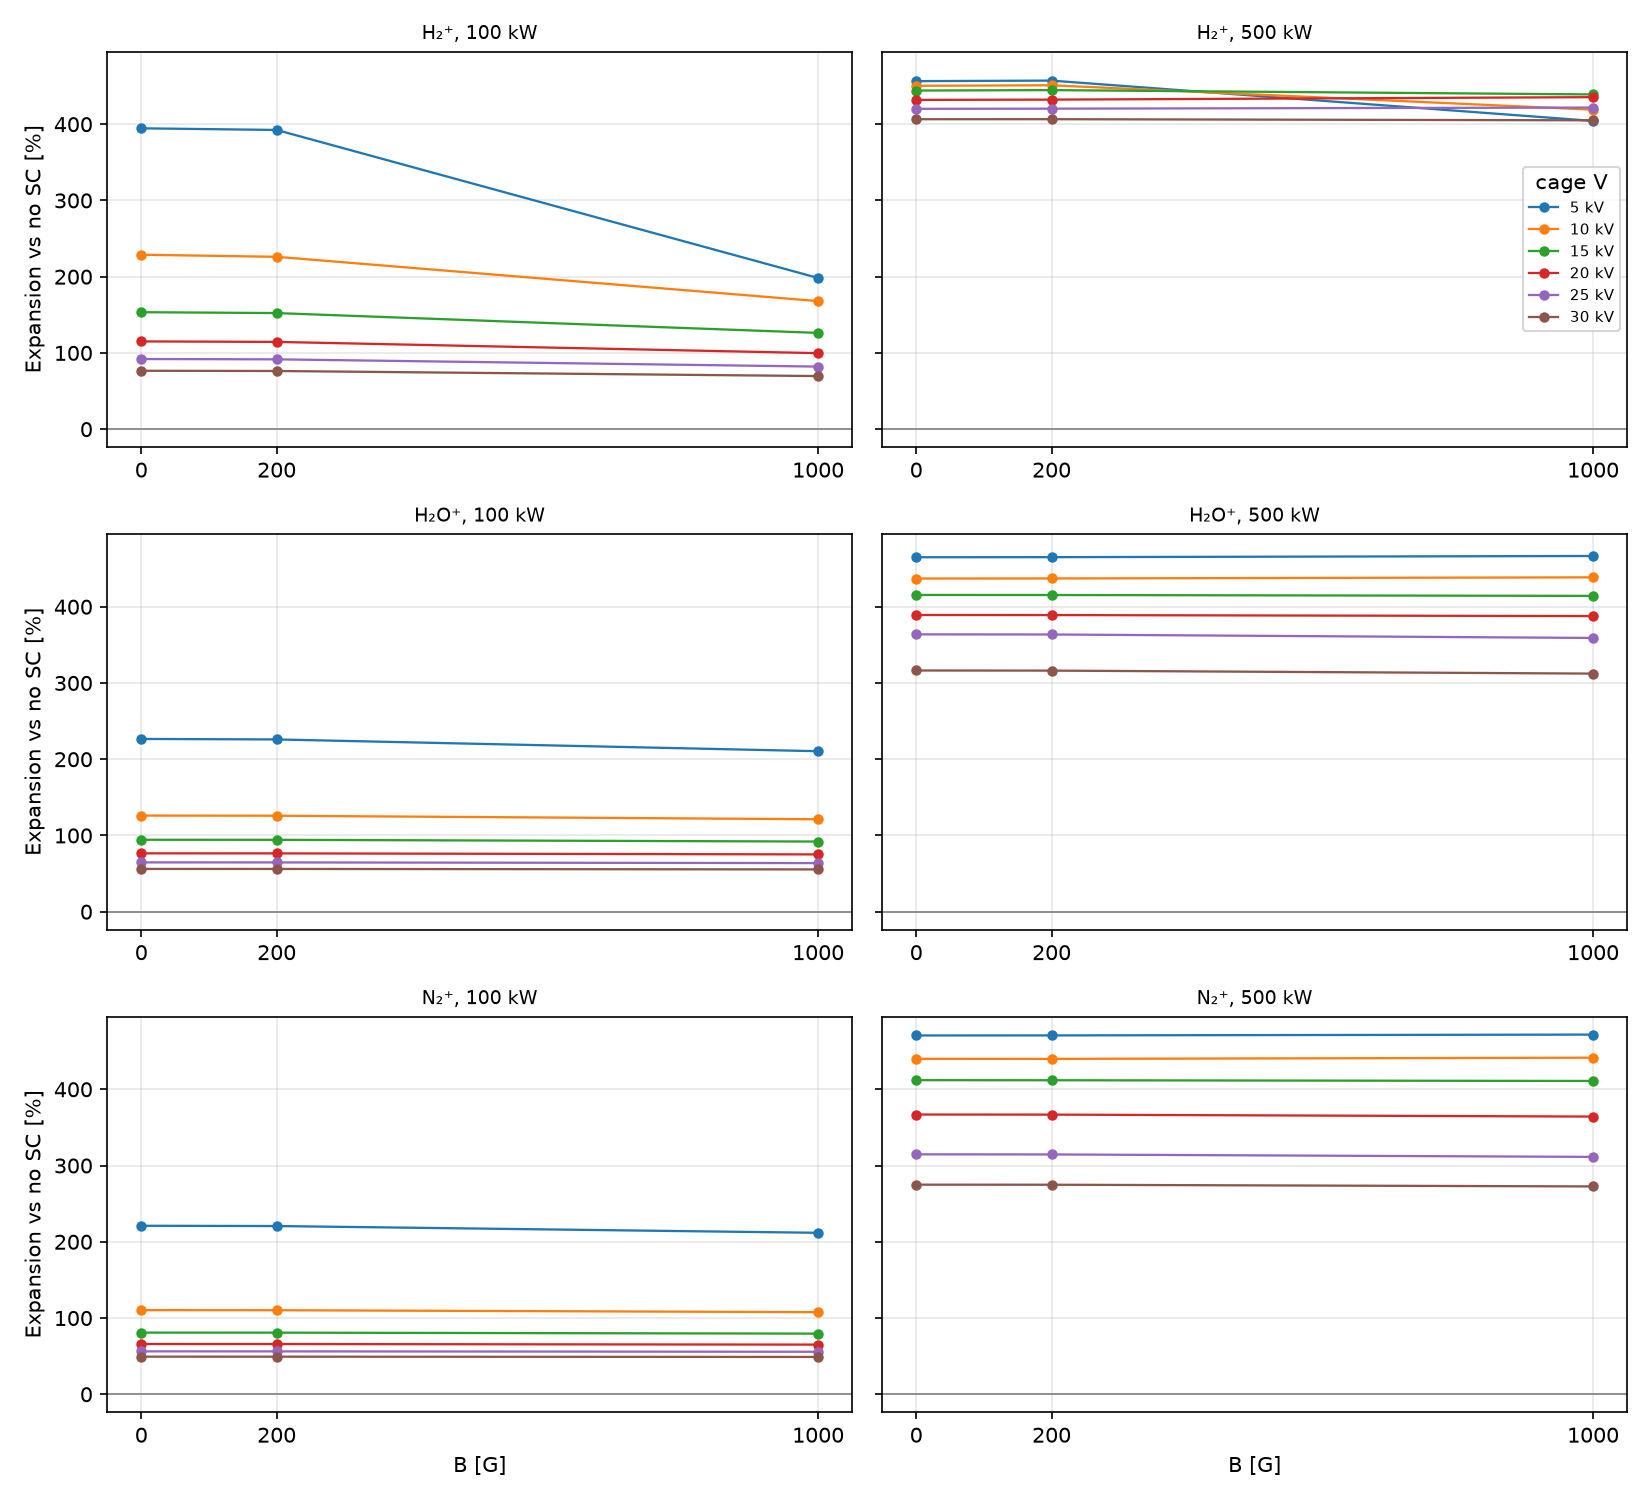
\includegraphics[width=0.98\textwidth]{csns_imode_voltage.png}
\caption{Ion-mode expansion versus guiding field at cage voltages from
$5$ to $30\,\mathrm{kV}$ (injection $10\,\mathrm{mm}$). Expansion
remains positive at every $V$.}
\label{fig:iV}
\end{figure}

Voltage is therefore a useful lever on the ion bias (a factor of about
three from $5$ to $30\,\mathrm{kV}$) but not a substitute for
correction or for electron-mode operation.

\subsection{Closed-orbit offset}
\label{sec:off}

Horizontal offsets of $+5$ or $+10\,\mathrm{mm}$ leave both electron
and ion widths unchanged at $100\,\mathrm{kW}$: the kick is centred on
the beam, in agreement with the ISIS statement that a linear scaling
correction holds within about $10\,\mathrm{mm}$ of the
axis~\cite{Pine2006}. A vertical offset of $\pm 5\,\mathrm{mm}$ changes
the drift length and therefore $\tau$; the ion expansion moves by a few
percent, in quantitative agreement with
$\sigma_m^2-\sigma_0^2\propto d$ ($0.5\%$ absolute). Electron recovery
at $300\,\mathrm{G}$ is preserved
($\lvert\Delta\rvert\le 0.65\%$ out to $\pm 10\,\mathrm{mm}$). At
$500\,\mathrm{kW}$ an uncorrected ion profile
($\sigma_m\approx 52\,\mathrm{mm}$) is clipped by the cage, and a
$10\,\mathrm{mm}$ horizontal offset then pulls the centroid by
$4\,\mathrm{mm}$. That is an aperture effect, not a failure of the
electron-mode operating point.

\subsection{Inversion of ion-mode widths}
\label{sec:inv}

Because the ion bias is large, smooth, and reproduced by a
one-dimensional kick model (Fig.~\ref{fig:kick}), $\sigma_0$ can be
recovered from $\sigma_m$ without changing the hardware. The procedure
is that used on the Fermilab Booster~\cite{Shiltsev2021}: identify the
time-of-flight peak; read $\sigma_m$ and the DCCT bunch charge $N$;
invert $\sigma_m=\sigma_0\,(1+\Delta)$ using a table
$\Delta(\sigma_0,N,V,\mathrm{species})$ generated by the kick model or
by Virtual-IPM, starting from $\sigma_0=\sigma_m$. CSNS has the same
inputs plus resolved time-of-flight peaks. The extraction column must
correspond to ions born in time with the bunch
(Fig.~\ref{fig:align}; $\mathrm{H}_2^+$ $+104\%$ at
$10\,\mathrm{mm}$, $100\,\mathrm{kW}$, $0\,\mathrm{G}$). Reported
accuracies on the Booster are $5$--$10\%$ on $\sigma_0$.

The inversion assumes that the profile has not reached the cage. At
$3\,\mathrm{mm}$ and $500\,\mathrm{kW}$ it has, and no table recovers
$\sigma_0$ from a wall-saturated r.m.s.\ width. Field-cage
non-uniformity---J-PARC reported a factor-of-two shrink from the
external map alone~\cite{Satou2010}---is not included and will have to
be folded in once the CSNS measured map is available.

\begin{figure}[ht]
\centering
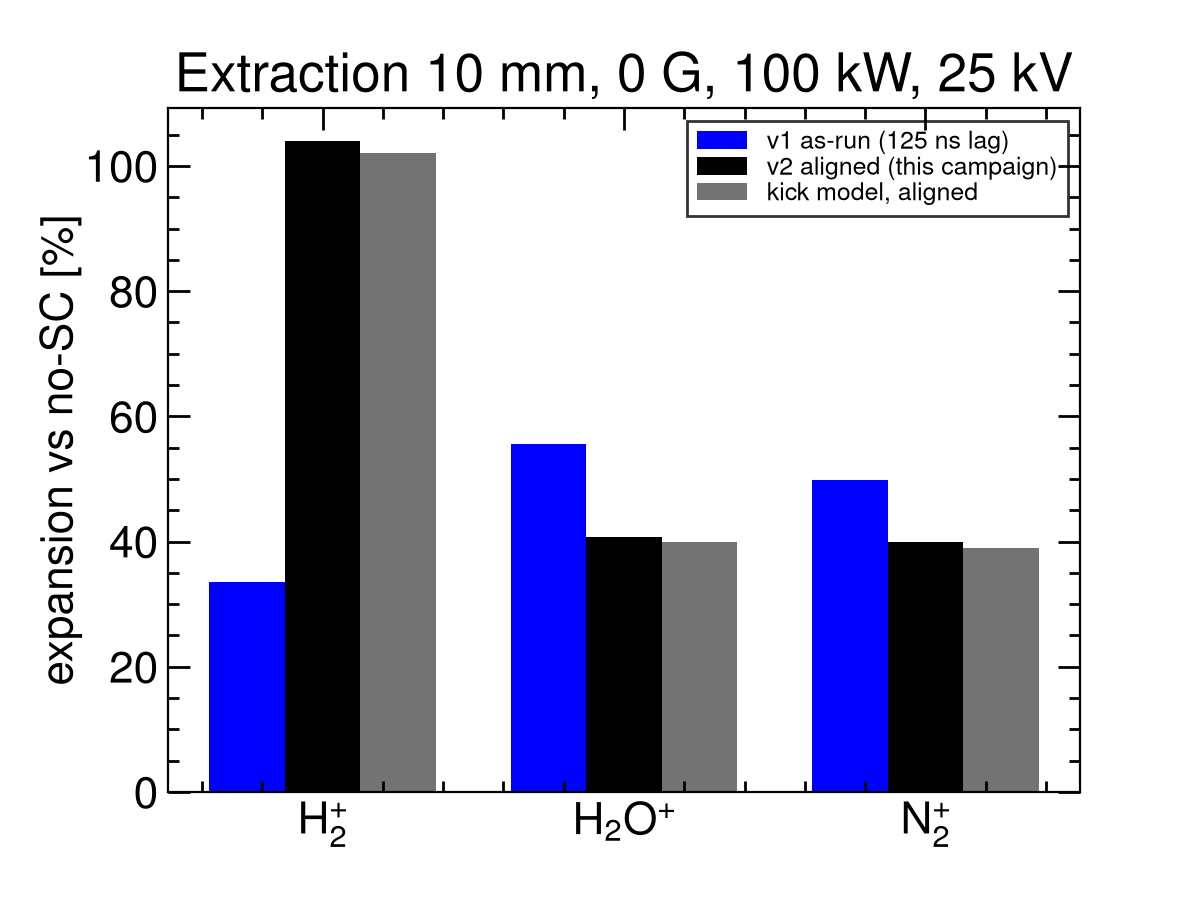
\includegraphics[width=0.72\textwidth]{csns_v2_aligned_extraction.png}
\caption{Extraction, $10\,\mathrm{mm}$, $0\,\mathrm{G}$,
$100\,\mathrm{kW}$, $25\,\mathrm{kV}$. Virtual-IPM with the ion born
in time with the bunch matches the kick model. These expansions are
the extraction ion widths to be inverted.}
\label{fig:align}
\end{figure}

\subsection{Summary}
\label{sec:sum}

Table~\ref{tab:eff} collects the efficiencies. Magnetic confinement at
$300\,\mathrm{G}$ is the only mitigation that returns a faithful
electron size. Cage voltage and look-up inversion address ion-mode
bias; neither brings an uncorrected $10\,\mathrm{mm}$,
$100\,\mathrm{kW}$ ion profile to the $10\%$ level.

\begin{table}[ht]
\centering
\caption{Efficiency of the mitigations examined. Residuals are quoted
for the families of Sections~\ref{sec:dist} and~\ref{sec:mit}.}
\label{tab:eff}
\begin{tabular}{p{3.4cm}p{5.4cm}p{5.4cm}}
\hline\hline
Mitigation & Electron mode & Ion mode \\
\hline
$B=300\,\mathrm{G}$
  & tens of percent $\to\lesssim 1\%$
    (all $P$, $V$, energy; $\sigma\ge 4\,\mathrm{mm}$)
  & --- \\
Design $B=0.1\,\mathrm{T}$
  & $3\,\mathrm{mm}$ on the diagonal; residual $\le 0.05\%$
  & --- \\
Raise $V$ ($5\to 30\,\mathrm{kV}$)
  & not a size fix at $B=0$; unused once $B\ge 300\,\mathrm{G}$
  & $+198\%\to +70\%$ ($\mathrm{H}_2^+$, inj.\ $10\,\mathrm{mm}$,
    $100\,\mathrm{kW}$); $10\%$ would require $\sim 380\,\mathrm{kV}$ \\
Orbit $\lesssim 10\,\mathrm{mm}$
  & $300\,\mathrm{G}$ still $\lesssim 1\%$
  & $\Delta x$: none; $\Delta y$: a few percent \\
Invert $\sigma_m=\sigma_0\,h(\sigma_0,N,V)$
  & unnecessary at $\ge 300\,\mathrm{G}$
  & recovers $\sigma_0$ if $N$ and species are known and the
    profile is inside the cage \\
\hline\hline
\end{tabular}
\end{table}

\section{Conclusions}
\label{sec:conc}

Space-charge distortion of the CSNS RCS IPM has been quantified with
uniform-field tracking and checked against a reduced kick model and
against the published electron-mode and ion-mode scalings.

Electrons experience an attractive kick that can focus or over-focus.
The resulting $\Delta(B)$ is a cyclotron-phase oscillation whose
envelope falls below $1\%$ at $300\,\mathrm{G}$ for every beam, power,
voltage and offset examined, and along the energy ramp. Size growth
with charge, and the non-monotonic $\sigma_m(\sigma_0)$ at $B=0$, both
disappear at that field. The design $0.1\,\mathrm{T}$ is a margin,
except for the smallest ($3\,\mathrm{mm}$) beams.

Ions experience a repulsive kick and are always collected with
$\sigma_m>\sigma_0$. The inflation scales as $N/\sigma_0^2$
(impulsive) and as approximately $1/V$, and matches the kick model to
$1\%$. Raising the cage voltage cannot bring a $10\,\mathrm{mm}$,
$100\,\mathrm{kW}$ ion profile to the $10\%$ level. A look-up
inversion can, provided the profile has not reached the wall.

The recommended operating point is therefore electron collection at
$B\gtrsim 300\,\mathrm{G}$. Ion time-of-flight should be used for
species identification; ion-mode widths should be reported only after
inversion. Once space charge is removed, the remaining electron-mode
systematic is hardware: microchannel-plate saturation after
$\sim 200\,\mu\mathrm{s}$, electromagnetic interference, secondary
electrons, and the real cage map~\cite{Rehman2024,Rehman2025,Xiao2026}.

\section*{Acknowledgements}

The hardware parameters follow Ref.~\cite{Rehman2026}. Tracking was
performed with Virtual-IPM~2.3.1~\cite{Vilsmeier2017}. This note is
prepared for internal review.

\begin{thebibliography}{99}

\bibitem{Huang2009}
W.~Huang \emph{et al.}, Ionization beam profile monitor designed for
CSNS, Proc.\ PAC'09, TH5RFP022.

\bibitem{Rehman2024}
M.A.~Rehman \emph{et al.}, Troubleshooting the ionization profile
monitor (IPM) for CSNS $1.6\,\mathrm{GeV}$ RCS, Proc.\ IBIC'24, WEP18.

\bibitem{Rehman2025}
M.A.~Rehman, Y.~Guo, Z.~Xu, X.~Nie, M.~Liu, B.~Zhang and R.~Yang,
Preliminary data analysis of an IPM prototype CSNS RCS, Proc.\ IBIC'25,
TUPMO41.

\bibitem{Rehman2026}
M.A.~Rehman \emph{et al.}, Fast residual gas ionization profile monitor
for bunch-by-bunch beam profile measurements in the CSNS rapid cycling
synchrotron, \emph{Nucl.\ Instrum.\ Methods} A \textbf{1092} (2026)
171809.

\bibitem{Xiao2026}
Xiao, Liu, Rehman and Yang, Optimization of the ion trap for secondary
electron suppression in the CSNS RCS IPM, IBIC'26, MOP026.

\bibitem{Vilsmeier2017}
D.~Vilsmeier, A modular framework for simulations of ionization profile
monitors, M.Sc.\ thesis (2017);
D.~Vilsmeier, P.~Forck and M.~Sapinski, Proc.\ IBIC'17, WEPCC07.

\bibitem{Vilsmeier2019}
D.~Vilsmeier, M.~Sapinski and R.~Storey, Space-charge distortion of
transverse profiles measured by electron-based ionization profile
monitors and correction methods, \emph{Phys.\ Rev.\ Accel.\ Beams}
\textbf{22} (2019) 052801.

\bibitem{Shiltsev2021}
V.~Shiltsev, Space-charge effects in ionization beam profile monitors,
\emph{Nucl.\ Instrum.\ Methods} A \textbf{986} (2021) 164744;
V.~Shiltsev \emph{et al.}, \emph{Phys.\ Rev.\ Accel.\ Beams}
\textbf{24} (2021) 044001.

\bibitem{Pine2006}
B.G.~Pine, S.J.~Payne, C.M.~Warsop \emph{et al.}, ISIS IPM studies,
Proc.\ EPAC'06 and DIPAC'07.

\bibitem{Forck2011}
P.~Forck \emph{et al.}, Ionization profile monitors --- IPM @ GSI,
Proc.\ DIPAC'11, TUPD51.

\bibitem{Satou2010}
K.~Satou \emph{et al.}, IPM systems for J-PARC RCS and MR, Proc.\
HB2010, WEO1C05.

\bibitem{Bartkoski2014}
D.A.~Bartkoski, C.~Deibele and Y.~Polsky, Design of an ionization
profile monitor for the SNS accumulator ring,
\emph{Nucl.\ Instrum.\ Methods} A \textbf{767} (2014) 379.

\bibitem{Levasseur2026}
S.~Levasseur \emph{et al.}, Detection of ionization electrons with
hybrid pixel detectors at the CERN Proton Synchrotron,
\emph{Nucl.\ Instrum.\ Methods} A \textbf{1081} (2026) 170845.

\bibitem{Marroncle2023}
J.~Marroncle \emph{et al.}, Proc.\ IBIC'23, WEP001;
F.~Benedetti \emph{et al.}, \emph{JINST} \textbf{15} (2020) T05007.

\end{thebibliography}

\end{document}
